\chapter{Reconstruções baseadas em fotogrametria}\label{cap:pontosdeinteresse}
%======================================================================================
%
\section*{Introdução}

A reconstrução 3D pelo método da estrutura do movimento, ou \emph{Structure from Motion} (\emph{SfM}). Tem como base a utilização de pontos de interesse
(\emph{features}), que são pontos ou áreas em comum entre as imagens usadas na reconstrução. Para encontrar estes pontos, diferentes algoritmos são empregados. 

A maioria dos métodos baseados em SfM e MVS (\emph{Multi-View Stereo}) tem uma abordagem similar e funcionam com os seguintes passos \ref{fig:sfmpipeline}:

\begin{itemize}
\item{Obtenção de imagens}
\item{Processamento dos parâmetros de câmera para cada imagem}
\item{Reconstrução da geometria 3D de uma cena com um conjunto de imagens e seus parâmetros correspondentes}
\end{itemize}

\begin{figure}[!h]
	\centering
	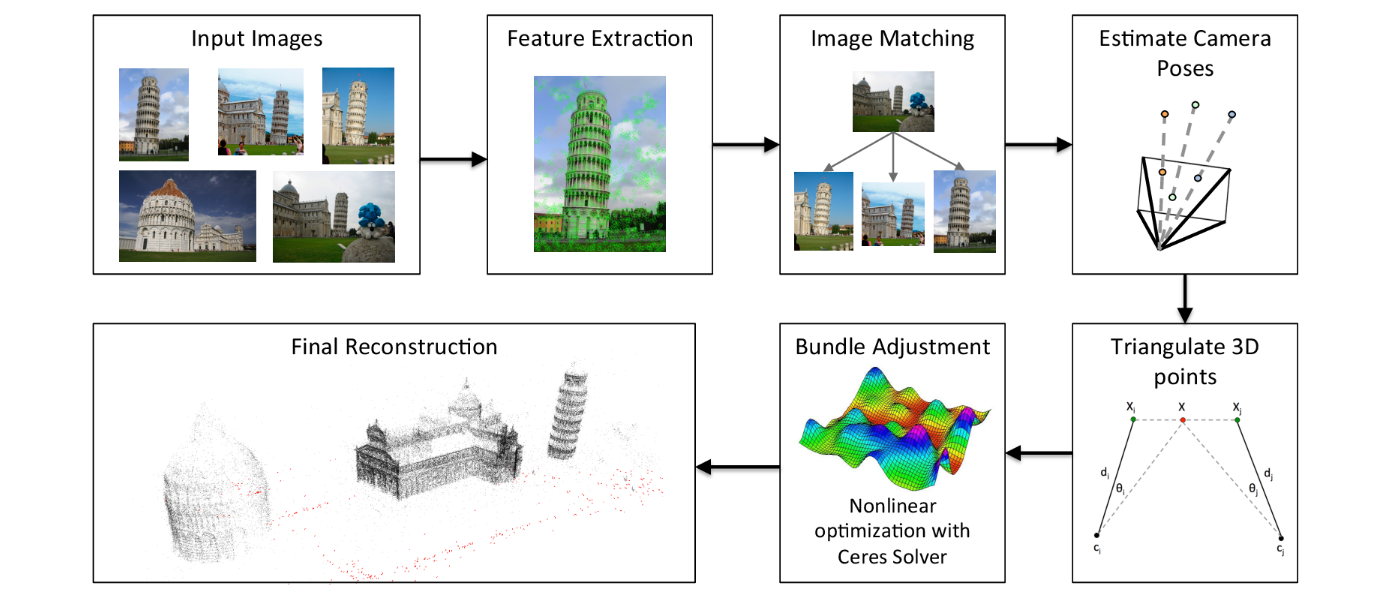
\includegraphics[width=0.5\linewidth]{figs/pipelinesfm.png}
	\caption{%
	Procedimento padrão da maioria dos sistemas baseados em SfM e MVS
	\protect\cite{theia-manual}.
	}\label{fig:sfmpipeline}
\end{figure}

Neste trabalho, abordaremos o uso de dois softwares baseados em MVS: o MVE~\cite{mve} e o VisualSfM~\cite{wu2011visualsfm}. Ambos utilizam os passos supracitados, que, posteriormente serão comentados. O que difere um do outro é a partir da etapa de reconstrução esparsa e densa, onde o MVE emprega um algoritmo de mapas de profundidade enquanto o VisualSfM utiliza um sistema baseado em \emph{Bundle Adjustment}. 

O passo de obtenção de imagens, será discutido no Capítulo de experimentos~\ref{sec:experiments}. Seguimos adiante com os algoritmos para processamento das imagens de entrada.

\section{Processamento dos parâmetros de câmera para cada imagem}

\section{ SIFT -- \emph{Scale Invariant Feature Transform}}

Primeiramente, utiliza-se o SIFT (algoritmo de detecção de pontos de interesse, invariante à escala e à transformações, como rotação, translação e iluminação da imagem, por exemplo).
O algoritmo pode ser dividido em cinco etapas, das quais:

\begin{itemize}
	\item{Deteccão de espaço-escala extremos -- \emph{Scale-space Extrema Detection}}
	\item{Localização de pontos-chaves -- \emph{Keypoint Localization}}
	\item{Atribuição de orientação -- \emph{Orientation Assignment}}
	\item{Descritor de pontos-chaves -- \emph{Keypoint Descriptor}}
	\item{Combinação de pontos-chaves -- \emph{Keypoint Matching}}
\end{itemize}


\subsection*{Detecção de espaço-escala extremos}\label{DiffGaussian}

% From the image above, it is obvious that we can't use the same window to detect keypoints with different scale. It is OK with small corner. But to detect larger corners we need larger windows. For this, scale-space filtering is used. In it, Laplacian of Gaussian is found for the image with various σ values. LoG acts as a blob detector which detects blobs in various sizes due to change in σ. In short, σ acts as a scaling parameter. For eg, in the above image, gaussian kernel with low σ gives high value for small corner while guassian kernel with high σ fits well for larger corner. So, we can find the local maxima across the scale and space which gives us a list of (x,y,σ) values which means there is a potential keypoint at (x,y) at σ scale.

Em casos com cantos pequenos, a detecção funciona bem. Porém, raramente utilizaremos a mesma janela para detectar pontos-chaves em imagens com diferentes escalas, pois utilizamos imagens grandes e, consequentemente, cantos grandes. Para isso, precisamos de janelas grandes também. 

Para resolver este problema, o filtro de escala-espaço é usado: o Laplaciano de Gaussiano (\emph{Laplacian of Gaussian} --  LoG). O LoG atua como um detector de particulas em diferentes tamanhos $\sigma$. (Onde $\sigma$ é o parâmetro de escala). Por exemplo, o núcleo Gaussiano com $\sigma$ baixo, tem como resposta um alto valor para um canto pequeno. Enquanto um núcleo gaussiano com alto $\sigma$, se encaixa bem para um canto maior. Com esta lógica, podemos encontrar um máximo local através da escala e o espaço, o que nos fornece uma lista de $(x,y \sigma)$, o que significa que existe um ponto-chave em potencial, com o par $(x,y)$ na escala $\sigma$.

% \begin{equation}
% LoG(x,y) = - \frac{1}{\pi \sigma ^4 }\left [ 1 - \frac{x^2+y^2}{2 \sigma ^2} \right ]e^{- \frac{x^2+y^2}{2 \sigma ^2}} 
% \end{equation}

Porém, como o LoG é um pouco custoso, computacionalmente. O SIFT utiliza um algoritmo aproximado do LoG, o DoG (Diferença de Gaussianos -- \emph{Difference of Gaussians}). O DoG é a diferença de um filtro Gaussiano de uma imagem, com dois valores diferentes de escala $\sigma$. 

Uma aplicação prática do filtro DoG é a sequência de imagens a seguir:

\begin{figure} [!h]
	\centering
	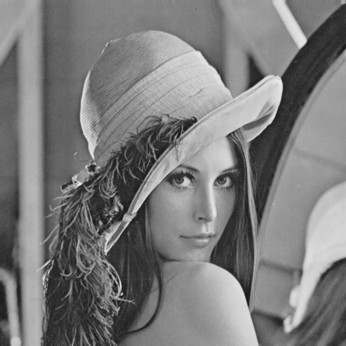
\includegraphics[width=0.45\linewidth]{figs/lena.jpg}(a)
	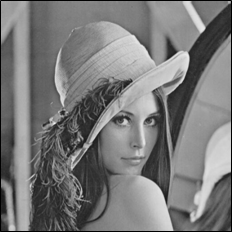
\includegraphics[width=0.45\linewidth]{figs/lenaSigma1.png}(b)
	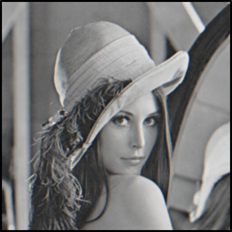
\includegraphics[width=0.45\linewidth]{figs/lenaSigma2.png}(c)
 	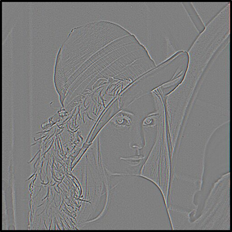
\includegraphics[width=0.45\linewidth]{figs/lenaDoG.png} (d)
	\caption{%
	É aplicado um filtro gaussiano na imagem original (a), com $\sigma$ = 1, tendo como resultado a imagem (b).
	Um outro filtro gaussiano é usado, porém, neste caso, o $\sigma$ = 2 (c). Após isso, subtrai-se (b) de (c), obtendo 
	o filtro DoG (d).
	}\label{fig:lenadog}
\end{figure}

Uma vez que o DoG é aplicado, as iamgens são utilizadas com o espaço e escala extremos. Por exemplo, na imagem \ref{fig:extrema}, um pixel é comparado com seus 8 vizinhos, assim como comparado com os 9 pixels na próxima escala e os 9 pixels na escala anterior. Se esse pixel é um local extremo, ele é um ponto-chave em potencial. Isto é, este ponto-chave é melhor representado nesta escala.

\begin{figure}
	\centering
	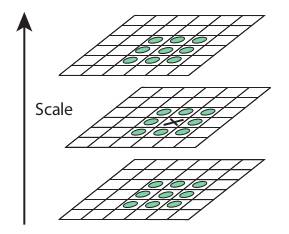
\includegraphics[width=0.45\linewidth]{figs/sift_local_extrema.jpg}
	\caption{%
	Exemplo de funcionamento de deteccão de espaço-escala extrema
	}\label{fig:extrema}
\end{figure}

No caso, as funções ficariam da seguinte forma: 

\begin{equation}
\label{eq:gaussiano}
	g_\sigma(x) = \frac{1}{2 \pi \sigma ^2} e^{-\frac{1}{2} \frac{x^T x}{\sigma ^2}}
\end{equation}

\begin{equation}
\label{eq:gaussianScaleSpace}
	I_\sigma = g_\sigma * I, \sigma >= 0
\end{equation}

\begin{equation}
\label{eq:LoG}
	\triangledown^2	g_\sigma(x)
\end{equation}

\begin{equation}
\label{eq:DoG}
	DoG_\sigma(o,s) = I_\sigma(o,s+1) - I_\sigma(o,s)
\end{equation}


Onde \ref{eq:gaussiano} é a função padrão do operador gaussiano (núcleo), a equação \ref{eq:LoG} é o operador LoG,  \ref{eq:DoG} é o operador DoG e $\triangledown^2$ é o operador Laplaciano.

\subsection*{Localização de pontos-chaves}

A localização dos pontos extremos pode cair em um extremo local e não global. Logo, após a utilização do DoG e com os pontos-chaves em potencial localizados, eles precisam ser refinados para melhorar o resultado. Para isso, são utilizadas Séries de Taylor na escala e no espaço, e, se a intensidade nesse extremo é menor que o valor limite, este é rejeitado.
%TODO: Ver isso 
Os \emph{frames} do SIFT (pontos-chaves) são extraídos baseados nos extremos locais (picos) a partir do DoG. Numericamente, extremos locais são elementos que possuem um menor (ou maior) valor em uma vizinhança em um espaço 3x3x3 (em escala e espaço).
Depois de extraídos, estes pontos são interpolados quadraticamente (este passo é muito importante, especialmente nas escalas de menor resolução, para ter uma localização precisa do ponto-chave na resolução completa). Finalmente, eles são filtrados para eliminar respostas de baixo contraste ou respostas próximas as bordas.

%Eliminating low contrast responses

Picos que são pequenos, na maior parte das vezes são gerados a partir de ruídos e necessitam ser descartados também. Isso é feito com uma comparação de valor absoluto do DoG no pico com o valor do pico limite e é descartado caso este valor é menor que o limite.


%Eliminating edge responses 

Para eliminar respostas em bordas, normalmente os picos mais rasos ou horizontais, são gerados por bordas e não possuem características estáveis, portanto estes picos precisam ser removidos. Para isso, dado um pico (x, y, $\sigma$), o algoritmo avalia a matriz Hessiana (x,y) do DoG na escala $\sigma$. Então é computado um valor para esta equação (\ref{eq:hessianaDoG}):

\begin{equation}
	v = \frac{( T_r \ D(x,y,\sigma))^2}{Det \ D(x,y,\sigma)}
	\label{eq:hessianaDoG}
\end{equation}
Onde, $T_r$ é o traço, ou seja, $T_r(H) = D_{xx} + D_{yy}$ e a matriz $D$ é do tipo
\[D = \begin{bmatrix}
	\frac{\partial ^2 DoG}{\partial x^2} & \frac{\partial ^2 DoG}{\partial x \partial y} \\ 
	\frac{\partial ^2 DoG}{\partial x \partial y} & \frac{\partial ^2 DoG}{\partial y^2} 
\end{bmatrix}
\]

No caso, v possui um valor mínimo (igual a 4) quando os autovalores da Jacobiana são iguais (pico curvado) e aumentam à medida que um dos autovalores aumenta e os outros permanecem baixos. Os picos são retidos se $v  < \frac{(t_e+1)(t_e+1)}{t_e}$ , onde $t_e$ é o limite da borda. 

\subsection{Atribuição de orientação}

Agora, uma orientação é atribuída a cada ponto-chave para obter a invariância à rotação da imagem. 
Uma vizinhança é obtida, dependente da escala, do gradiente da magnitude \ref{eq:magnitudeSIFT} e da direção \ref{eq:direcaoSIFT} (usando diferenças finitas), ao redor da localização do ponto-chave. 

\begin{equation}
	m(x,y) = \sqrt{(L(x+1,y)-L(x-1,y))^2 + (L(x,y+1)-L(x,y-1)^2)}
	\label{eq:magnitudeSIFT}
\end{equation}

\begin{equation}
	\theta = tan^{-1} \left( \frac{(L(x,y+1)-L(x,y-1)}{(L(x+1,y)-L(x-1,y)}\right)
	\label{eq:direcaoSIFT}
\end{equation}

Então, um histograma de 36 orientações (\emph{bins}) cobrindo 360 graus é criado. Onde ele é ponderado pelo gradiente da magnitude e por uma janela Gaussiana circular onde $\sigma$ vale $1.5$ em relação à escala do ponto-chave \ref{fig:histogramaOrientado}.

\begin{figure} [!h]
	\centering
	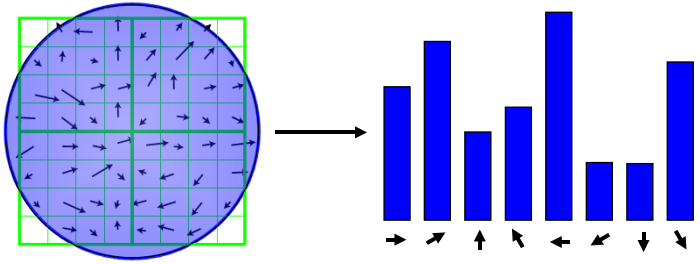
\includegraphics[width=0.45\linewidth]{figs/histogramaOrientado.png}
	\caption{%
	Exemplo do resultado obtido do histograma orientado
	}\label{fig:histogramaOrientado}
\end{figure}

O ponto mais do histograma é obtido e qualquer pico acima de 80\% é considerado no cálculo da orientação. 
Pontos-chaves são criados com a mesma localização e escala, mas em diferentes direções, o que contribui para a establidade da correspondência.

\subsection*{Descritor de pontos-chaves}

Com os pontos-chaves criados a partir do histograma orientado, cria-se agora o descritor de pontos-chaves.

Uma vizinhança 16x16 ao redor do ponto-chave é escolhida e esta mesma vizinhaça é dividida em 16 sub-blocos 4x4. Para cada bloco, um histograma orientado com 8 \emph{bin} é criado. Logo, temos 128 valores válidos de \emph{bin}. Esses valores são representados em forma de vetor para expressar o descritor de pontos-chaves \ref{fig:descritorKeypoint}. 

Além disso, são tomadas algumas medidas para deixar o descritor mais robusto,como, por exemplo, invariante à luminosidade, rotação, etc.

\begin{figure} [!h]
	\centering
	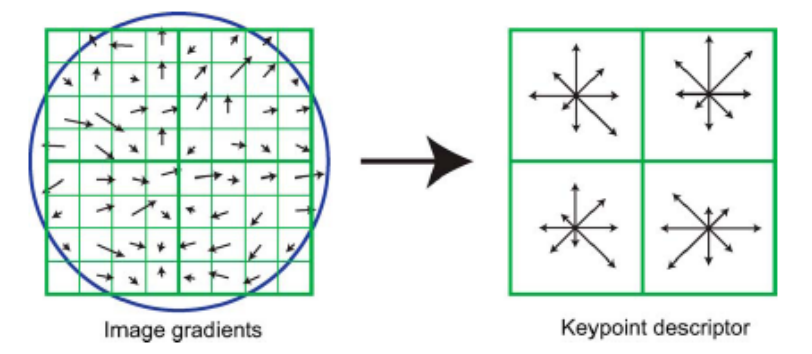
\includegraphics[width=0.45\linewidth]{figs/descritorKeypoint.png}
	\caption{%
	Exemplo de um descritor de pontos-chaves, com uma matriz 2x2 e uma região 8x8
	}\label{fig:descritorKeypoint}
\end{figure}

\subsection*{Combinação de pontos-chaves}

Pontos-chaves entre duas imagens são combinados a partir da identificação da vizinhança mais próxima. Mas, em alguns casos, a segunda combinação mais próxima pode ser parecida com a primeira. Isso se dá por ruídos presentes nas imagens ou algo assim. 

Nesse caso, a razão da distância mais próxima para a segunda distância mais próxima é utilizada. Se essa razão for maior que 0.8, essa combinação é descartada.
Esse método elimina cerca de 90\% de combinações falsas, enquanto descarta apenas cerca de 5\% de combinações corretas.

\section {Triangulação -- \emph{Full pair-wise image matching}}

Com os pontos de interesse (\emph{features}) extraídos, podemos agora fazer a triangulação entre os pontos das imagens.

A triangulação nada mais é que uma estimativa de um ponto em 3 dimensões, dado pelo menos duas câmeras conhecidas, onde, cada câmera com a projeção do \emph{feature} correspondente àquele ponto 3D \ref{fig:triangulacao}.

\begin{figure} [!h]
	\centering
	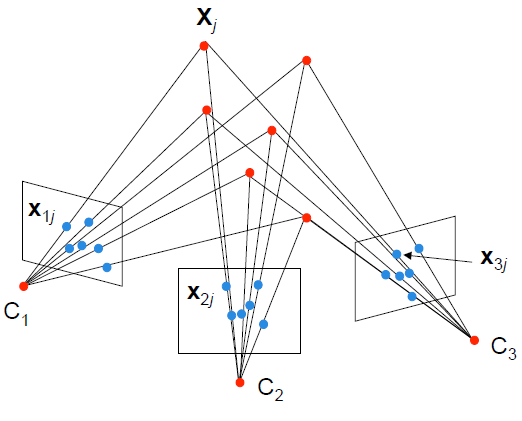
\includegraphics[width=0.45\linewidth]{figs/triangulacao.png}
	\caption{%
	Uma triangulação utilizando um ponto qualquer, $X_j$. Onde cada câmera $C_1, C_2, C_3$ possui um \emph{feature} correspondente a cada uma delas, respectivamente, $X_{1j}, X_{2j}, X_{3j}$.
	}\label{fig:triangulacao}
\end{figure}

Infelizmente, não é tão simples assim. Existem muitos fatores que contribuem para aumentar a dificuldade da triangulação: ruídos, posição das câmeras, o feixe das projeções não se encontram no mesmo ponto 3D, não se tem informação da projeções nas câmeras, dentre outros. Entretanto, existem diversos algoritmos para resolução de cada um dos problemas enfretados. 

Com a extração dos \emph{features} das imagens selecionadas, as próximas etapas da reconstrução para um dos sistemas se diferem, e a partir de agora, faremos abordagens individuais para cada um deles.


\section{MVE -- \emph{Multi-View Reconstruction Environment}}\label{sec:mve}
%======================================================================================
%
\subsection*{Introdução}
Um dos sistemas de pesquisa de ponta mais utilizados para a técnica de reconstrução densa é o MVE --
\emph{Multi-View Reconstruction Environment}~\cite{mve}. Este algoritmo utiliza
fotos e produz uma malha triangular superficial como resultado. Diferentemente
das reconstruções baseadas nas geometrias das imagens, o MVE é focado na
reconstrução multi-escala, um quesito importante na reconstrução de esculturas e
acervo cultural. Portanto, com esta técnica é possível reconstruir grandes
volumes de dados, contendo regiões detalhadas em alta resolução, em comparação
com o resto da cena. O sistema ainda possui uma interface gráfica para uma
reconstrução baseada no SfM, amigável ao usuário e conhecida como UMVE, que
permite a visualização e inspeção das imagens, mapas de profundidade e
renderizar cenas e malhas 3D. Sua base de operação é basicamente
\ref{fig:mvepipeline}:
\begin{enumerate}
\item{Estrutura por Movimento -- \emph{Structure-from-Motion} (SfM)}

\begin{itemize}
\item{
Reconstrói os parâmetros externos da câmera (posição e orientação) e seus
parâmetros internos de calibração (distância focal e distorção radial), encontrando correspondências
esparsas, mas estáveis entre as imagens.
}
\end{itemize}

\item{Estereoscopia multiocular -- \emph{Multi-View Stereo} (MVS)}
\begin{itemize}
\item{
Utiliza a posição estimada das câmeras, encontrando as correspondências visuais
nas imagens. Estas correspondências são trianguladas, produzindo a informação
3D, e, consequentemente a reconstrução 3D densa.
} 
\end{itemize}
\item{Reconstrução de superfícies -- \emph{Surface Reconstruction}}
\begin{itemize}
\item{
Tem como entrada uma densa nuvem de pontos, ou mapas de profundidade
individuais. Produz uma malha superficial globalmente consistente.
}
\end{itemize}
\end{enumerate}

\begin{figure}[!h]
	\centering
	%   \includegraphics[width=1.0\linewidth]{figs/3d-curve-sketch/system-diagram.eps}
	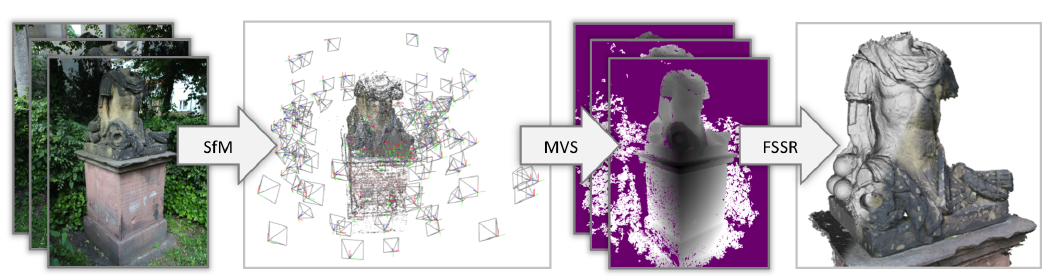
\includegraphics[width=\linewidth]{figs/mvepipe.png}
	\caption{%
  Funcionamento do MVE. Começando com múltiplas imagens, técnicas SfM são
  empregadas para recontruir os parâmetros das câmeras e os conjuntos de pontos
  esparsos. Mapas de profundidade são computados para cada imagem usando o MVS.
  Finalmente, uma malha colorida é extraída da união de todos os mapas de
  profundidade usando um algoritmo de aproximações de reconstruções de
  superfícies, FSSR -- \emph{Floating Scale Surface Reconstruction}.
	\protect\cite{mve}
	}\label{fig:mvepipeline}
\end{figure}

Como não existem muitas opções para algoritmos de SfM, o MVE permite a
utilização de \emph{softwares} externos como o
\emph{Bundler}~\cite{snavely2010bundler} ou o prório \emph{VisualSfM} para esta
etapa.  Tendo o SfM feito, partimos para o MVS. Com os parâmetros
de câmera conhecidos, a reconstrução densa geométrica é feita. Existem diversos
algoritmos para a reconstrução densa; o MVE utiliza um algoritmo
próprio, bastante popular, feito por um de seus criadores, Michael
Goesele~\cite{goesele2007multi}, que reconstrói um mapa de profundidade para
cada foto. 

Embora abordagens baseadas em mapeamentos de profundidade produzam uma grande
quantidade de redundâncias, (isso se dá por causa das inúmeras fotos que são
sobrepostas e possuem partes similares da mesma cena), este algoritmo é
altamente escalável para grandes cenas, pois apenas um pequeno conjunto de fotos
vizinhas é necessário para a reconstrução. Outra vantagem da utilização dos
mapas de profundidade como representação intermediária é que a geometria é
parametrizada em seu domínio natural, e os dados por foto (como a cor, por
exemplo) estão diretamente acessíveis nas imagens.

%Essa redundância excessiva nos mapas de profundidade pode ser pesado. Não com
%relação ao armazenamento, mas na questão do processamento computacional exigido
%nos mapas. Porém, esta abordagem foi capaz de produzir uma geometria detalhada e
%superar o ruído nos mapas de profundidade individuais.

\subsection*{Guia de reconstrução com o MVE}
Existem algumas recomendações para se ter uma boa reconstrução com o MVE~\cite{pipelinemve,mve}.
Um bom conjunto de dados é gerado se algumas regras simples forem seguidas:

\begin{itemize}

\item{Para que o algoritmo MVS consiga fazer uma triangulação com qualquer
  posição 3D, o conjunto de dados terá que ter, no mínimo, cinco fotos.}

\item{As fotos devem ser tiradas com uma boa quantidade de sobreposição. A menos que o conjunto de dados se torne muito grande, uma grande quantidade de fotos não prejudicará a qualidade. 
Mas terá uma compensação do sistema, no que diz respeito à qualidade e desempenho.}

\item{Para a triangulação funcionar, é necessário que tenha o efeito de paralaxe
    \ref{fig:parallax}.}

\item{A câmera deverá ser reposicionada, de preferência.}

\end{itemize}

\begin{figure} [!h]
	\centering
	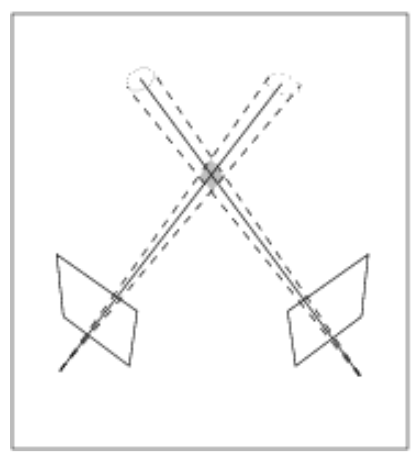
\includegraphics[width=0.2\linewidth]{figs/parallaxA.png}(a)
	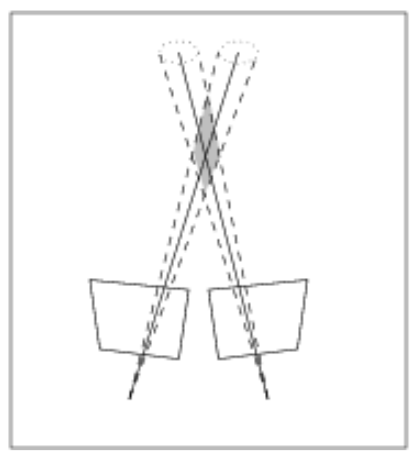
\includegraphics[width=0.2\linewidth]{figs/parallaxB.png}(b)
	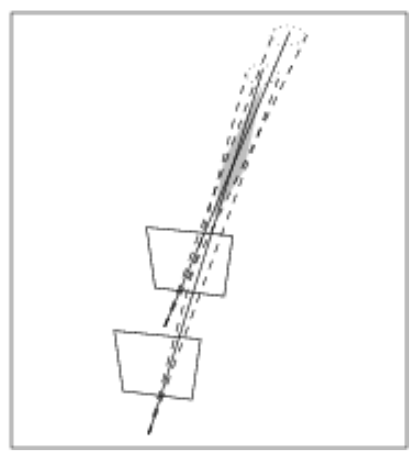
\includegraphics[width=0.2\linewidth]{figs/parallaxC.png}(c)
	\caption{%
  Com espaçamento grande entre câmeras, a informação extraída das
  imagens em comum é menor (a). Se a angulação do efeito de paralaxe for
  baixa, terá a mesma informação sobre um ponto 3D (c).
  Nesses casos, a reconstrução pode ser incerta. Para que
  o efeito paralaxe tenha maior proveito das imagens, alguns autores argumentam que
  câmeras devem estar dispostas como (b), de forma a extrair uma boa
  quantidade e qualidade de informações do ponto.
  \protect\cite{3DCompVision2Didier}
	}
	\label{fig:parallax}
\end{figure}

% Creating a scene: A view is a container that contains per-
% viewport data (such as images, depth maps and other data).
% A scene is a collection of views, which make up the dataset.
% A new scene is created using either the graphical interface of
% our software, UMVE, or the command line tool makescene.
% Technically, the scene appears as a directory in the file sys-
% tem (with the name of the dataset). It contains another direc-
% tory views/ with all views stored as files with the extension
% .mve. Creating a new scene will solely create the views/
% directory for now. Importing photos will create a .mve file
% for every photo. This process will also import meta informa-
% tion from the images (EXIF tags), which is required to get
% a focal length estimate for every photo. If EXIF tags are not
\subsubsection*{Criando uma cena}

Uma vista (\emph{view}) no MVE contém dados por \emph{viewport} (como imagens,
mapas de profundidade ou outros dados). Uma cena é uma coleção de vistas que
formam um conjunto de dados (\emph{dataset}). Uma nova cena pode ser criada
utilizando a interface gráfica UMVE, Figura~\ref{fig:umve:gui}, ou por linha de
comando (\emph{makescene}).  Tecnicamente, a cena é criada como um diretório no
sistema de arquivos (com o nome do conjunto de dados). Este, por sua vez, contém
outro diretório (\emph{views}), com todas as vistas guardadas com uma extensão
de arquivos em\ \texttt{.MVE}.

Criar uma nova cena também criará apenas o diretório (\emph{views}) vazio. A
importação de fotos criará arquivos .MVE para cada foto. Esse processo importará
metadados provenienteas das imagens (\emph{tags} EXIF), que é necessário para
estimar a distância focal para cada foto a partir do modelo de câmera gravado em
determinados tipos de arquivos de imagem. Caso estes meta-dados não estejam
disponíveis, uma distância focal padrão é assumida pelo sistema, porém se essa
distância adotada for uma péssima suposição, com relação ao conjunto de dados
utilizado, podem acontecer erros no SfM.

\begin{figure}[!h]
	\centering
	%   \includegraphics[width=1.0\linewidth]{figs/3d-curve-sketch/system-diagram.eps}
	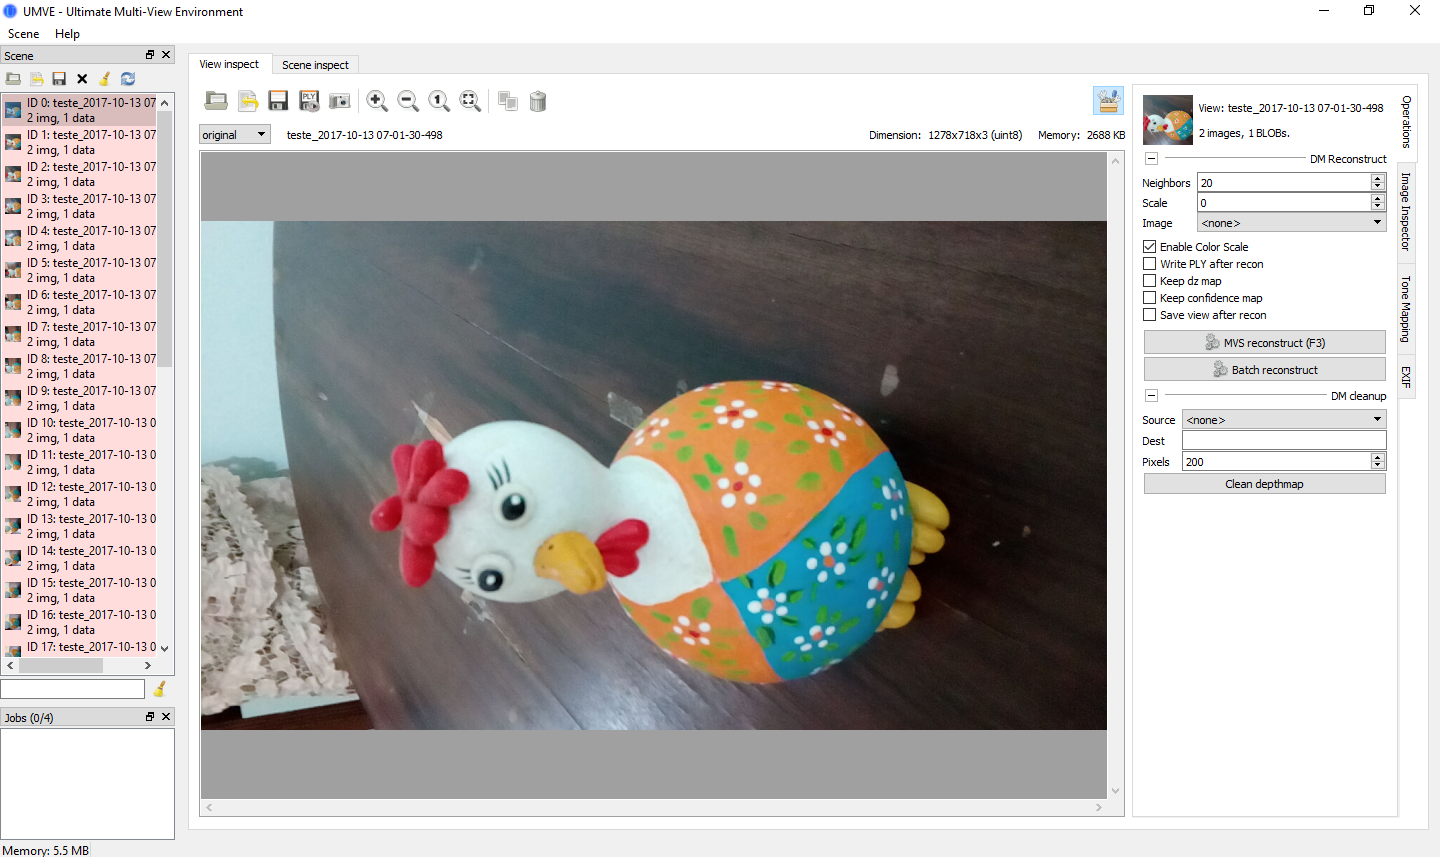
\includegraphics[width=\linewidth]{figs/umve1.png}
	\caption{%
	Interface gráfica (UMVE)%\cite{Cui:Theobalt:etal:PAMI2013,Pajdla:etal:ICCV2011}.
	}\label{fig:umve:gui}
\end{figure}
% SfM reconstruction: The SfM reconstruction can be con-
% figured and started using UMVE, or the command line tool
% sfmrecon. The UI guides through feature detection, pairwise
% matching and incremental SfM. What follows is the SfM re-
% construction starting from an initial pair, and incrementally
% adding views to the reconstruction. Finally, the original im-
% ages are undistorted and stored in the views for the next step.
% Figure 8 shows a rendering of the SfM reconstruction with
% the sparse point cloud and the camera frusta. Note how dense
% the frusta are spaced around the object to achieve a good re-
% construction.
\subsection*{Reconstrução SfM}

Pode ser configurada e iniciada a SfM usando a interface gráfica UMVE ou por linha de
comando (\texttt{sfmrecon}). A interface guia através da detecção de
\emph{features}, casamento de todos os pares de imagens (\emph{pairwise matching}) e uso
incremental do SfM. A reconstrução SfM começa a partir de um
par inicial, e adiciona, de forma incremental, mais vistas à
reconstrução~\ref{fig:mvesfm}.

\begin{figure}[!h]
	\centering
	%   \includegraphics[width=1.0\linewidth]{figs/3d-curve-sketch/system-diagram.eps}
	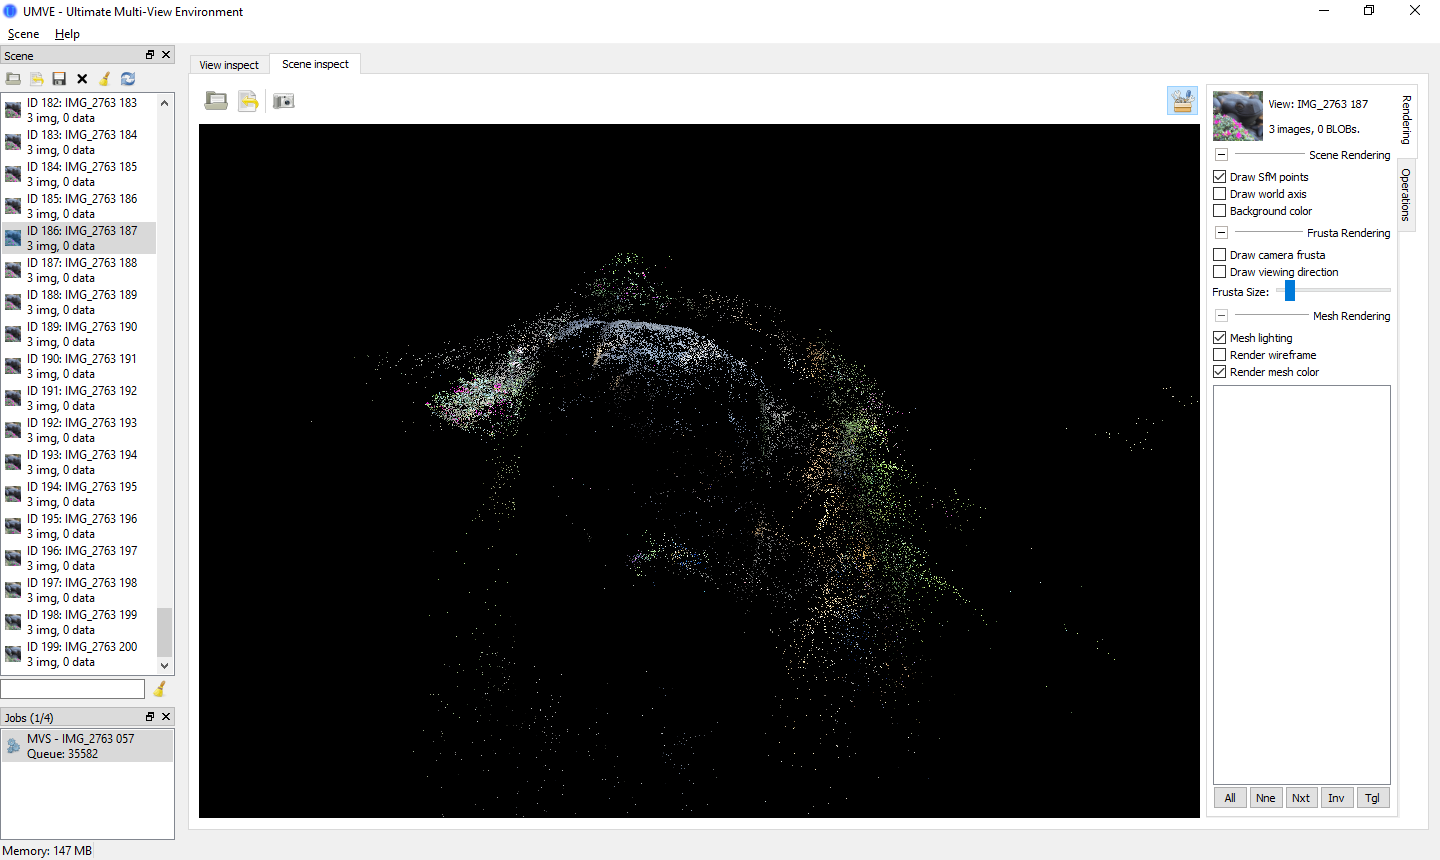
\includegraphics[width=\linewidth]{figs/umve5sfm.png}
	\caption{%
  Reconstrução de nuvem de pontos gerada a partir de
  SfM do MVE%\cite{Cui:Theobalt:etal:PAMI2013,Pajdla:etal:ICCV2011}.
	}\label{fig:mvesfm}
\end{figure}


%
%MVS reconstruction: Given images with camera parameters,
%dense geometry is reconstructed using MVS. This can
%be done with either UMVE or the command line tool dmrecon.
%The most important parameter is the resolution level at
%which depth maps are reconstructed. A level of 0, or L0, reconstructs
%at the original image size, L1 corresponds to half
%the size (quarter the number of pixels), and so one. Looking
%at the resolution of recent digital cameras, a full-size L0
%reconstruction is rarely useful as finding dense correspondences
%gets more difficult, often leading to sparser depth
%maps at much higher computational cost. Using smaller images
%(we often use L2), the process is faster and depth maps
%become more complete. See Figure 9 for a depth map computed
%at L2.
\subsubsection*{Estereoscopia Multiocular -- \emph{Multi-View Stereo} (MVS)}

Usando as imagens junto com os parâmetros obtidos das câmeras, é possível
reconstruir a geometria densa utilizando o MVS. Isso pode ser feito utilizando a
interface gráfica (UMVE) ou por linha de comando (\emph{dmrecon}).
O parâmetro mais importante é o nível de resolução em que os mapas de
profundidade são reconstruídos: Caso seja nível 0 (ou L0), a reconstrução é
feita usando o tamanho original das imagens. Se for nível 1 (ou L1), a
reconstrução corresponde à metade do tamanho (um quarto dos números de pixels),
e assim por diante.

Com a alta resolução das câmeras atuais, uma reconstrução L0 é raramente usada, pois
geram mapas de profundidade mais dispersos com um custo computacional elevado, o
que acarreta em dificuldades para encontrar as correspondências densas das
imagens. Geralmente utiliza-se o L2, pois o processo é mais rápido, gerando
mapas de profundidades completos, já que utiliza resoluções menores, Figura~\ref{fig:mvedepth}.

\begin{figure}[!h]
	\centering
	%   \includegraphics[width=1.0\linewidth]{figs/3d-curve-sketch/system-diagram.eps}
	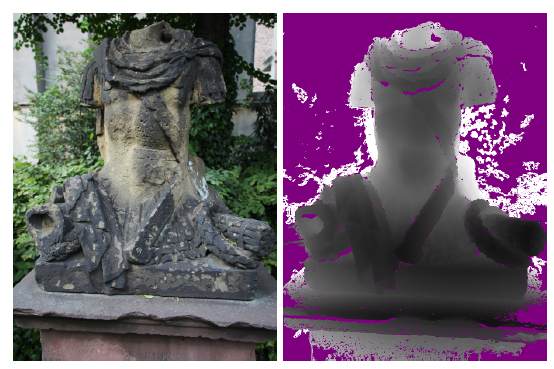
\includegraphics[width=0.7\linewidth]{figs/mvedepth.png}
	\caption{%
  Uma imagem de entrada (esquerda) e correspondência em mapas de
  profundidade (direita), em roxo as partes sem nenhum mapa naquela região~\protect\cite{mve}.
	}\label{fig:mvedepth}
\end{figure}

O MVS pode ser dividido em duas partes:
\begin{itemize}
\item {Uma estrutura regional-crescente que tem uma fila de candidatos
  correspondentes, $Q$, ordenada pelas localizações dos pixels na câmera
acrescido de seus valores para profundidade e normais;}
\item {Um sistema de correspondências que leva um candidato correspondente como
  entrada e calcula profundidade, normal e uma confiança de correspondência
usando vistas vizinhas fornecidas pela seleção de exibição local. Se a
correspondência for bem sucedida, os dados são armazenados em mapas de
profundidade, normais e de confiança e os pixels vizinhos na câmera são
adicionados como novos candidatos a $Q$.}
\end{itemize}

\subsubsection*{Reconstrução de Superfícies -- \emph{Surface Reconstruction}}

Utiliza-se o programa em linha de comando \texttt{scene2pet}, que combina todos os mapas de
profundidade em uma única e grande nuvem de pontos. Nesta fase, um valor de
escala é atribuído a cada ponto, que indica o tamanho atual da região da
superfície na qual o ponto foi mensurado. Esta informação adicional permite o
uso de várias propriedades benéficas usando a abordagem de reconstrução de
superfície por FSSR~\cite{fuhrmann2014floating}.  A seguir, as ferramentas
FSSR calculam uma representação volumétrica de escala múltipla a partir dos
pontos (na qual não precisa de nenhum ajuste de parâmetros explícitos) e uma
malha final é extraída. Esta malha pode parecer desordenada devido a regiões não
confiáveis e a componentes isolados, oriundos de medidas imprecisas. Logo, a
malha é limpa, retirando pequenos componentes isolados e regiões não confiáveis
da superfície. 

% Experiência com o MVE: A utilização do software é bem intuitiva, seja por linha de comando ou pela interface gráfica (neste modo, fica mais fácil visualizar cada etapa da reconstrução). Amplamente configurável, podendo escolher a vizinhança, escala, manter o mapa de profundidade, ver os dados \emph{EXIF} de cada imagem, dentre outras configurações.

% Entretanto, para a aplicação proposta neste projeto, não é muito interessante, visto que ele utiliza a informação das câmeras (\emph{EXIF}) e das imagens e, como as imagens empregadas na reconstrução são, tecnicamente, vídeos cortados em determinados \emph{frames}, não é possível obter a informação das câmeras \ref{fig:mveexif}, logo o software não tem tanta aplicabilidade neste caso, pois recai no problema dos parâmetros padrões adotados para as câmeras não serem bons o suficiente para estes conjuntos de dados, a menos que sejam tiradas fotos sequenciais de alguma escultura ou objeto que se deseja gerar a reconstrução densa, pois dessa forma, as informações necessárias das câmeras estarão armazenadas.

% \begin{figure}[!h]
% 	\centering
% 	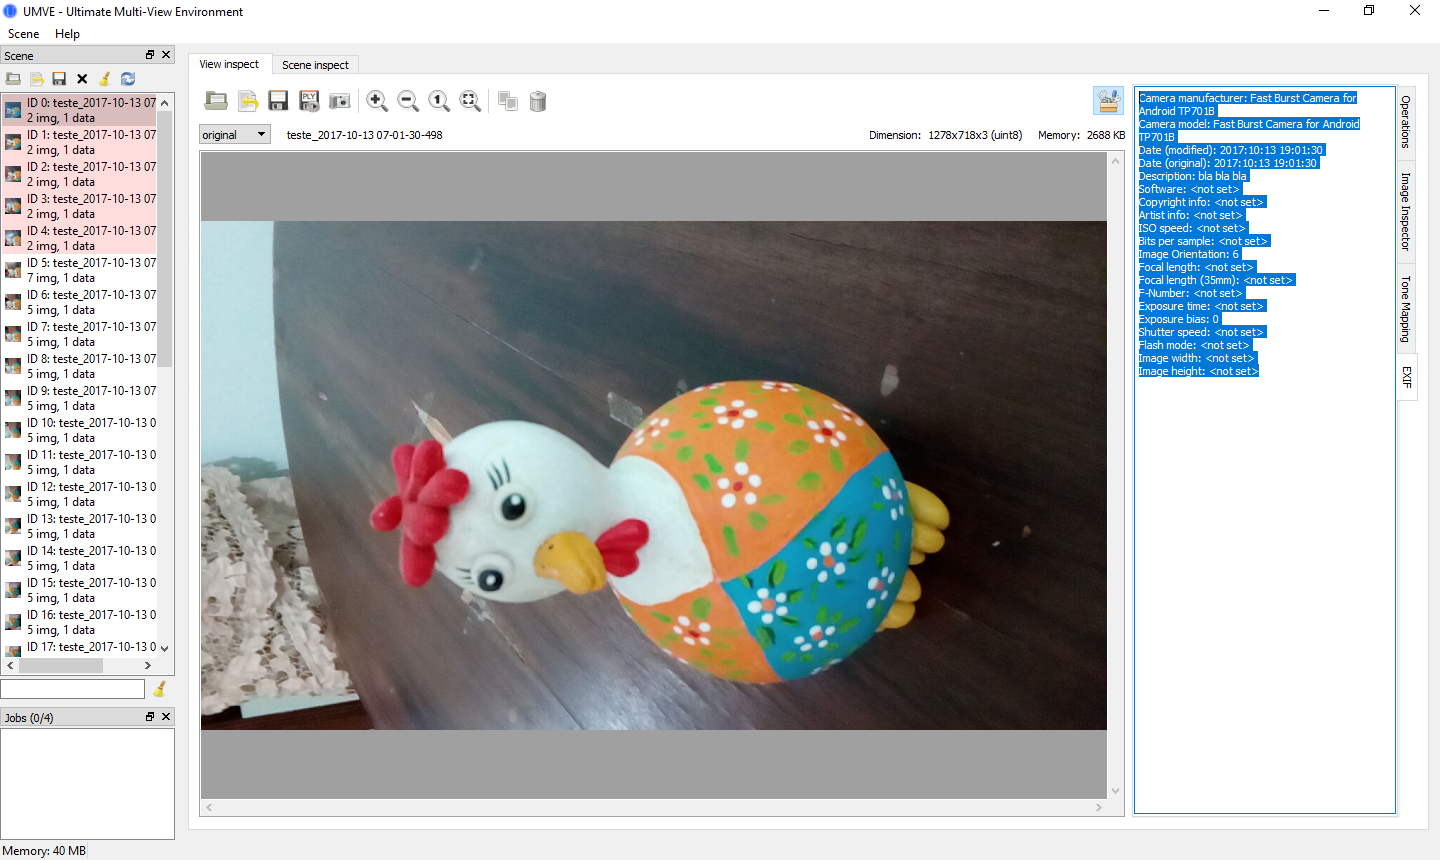
\includegraphics[width=0.5\linewidth]{figs/exifumve.png}(a)
% 	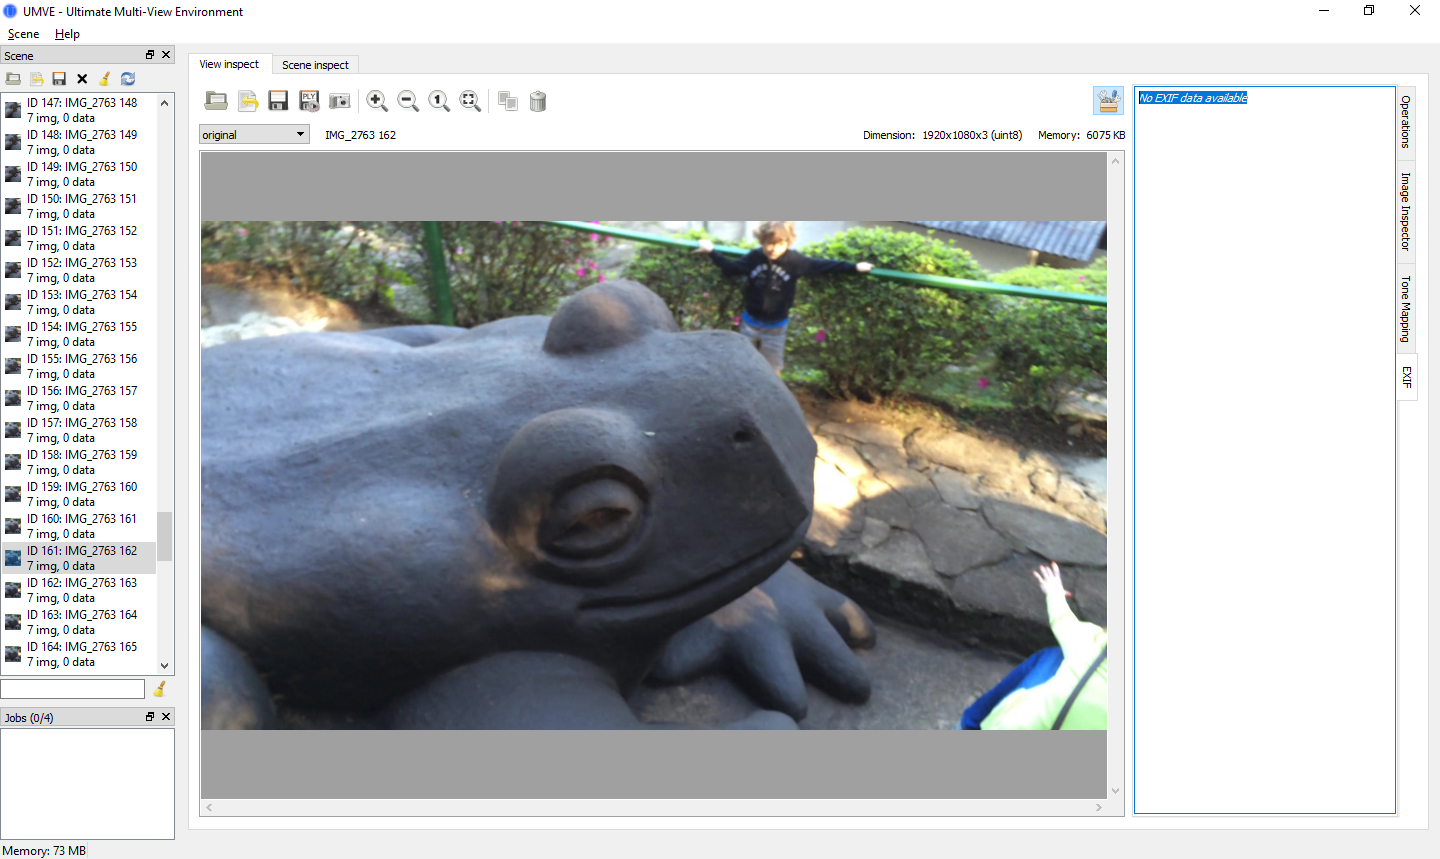
\includegraphics[width=0.5\linewidth]{figs/exifsemumve.png}(b)
% 	\caption{%
% 	A figura (a) é um exemplo onde a imagem possui dados na extensão \emph{EXIF} (destacado em azul). Ao passo que a figura (b) é um frame de um vídeo, que não possui os dados das câmeras (destacado em azul).
% 	%\cite{Cui:Theobalt:etal:PAMI2013,Pajdla:etal:ICCV2011}.
% 	}\label{fig:mveexif}
% \end{figure} 

% Com isso em mente, foi gerada uma reconstrução de um vídeo gravado de uma escultura no Jardim do Nêgo. O  vídeo foi cortado em \emph{frames} onde foram geradas 200 imagens base. 

% A partir disso, foi executado, todos os passos de uma reconstrução utilizando o MVE, de forma que, foram utilizadas as duas opções, tanto por linha de comando, quanto pela interface gráfica (UMVE).

% Pela interface gráfica, o processo todo de reconstrução foi rápido (cerca de 30 minutos) \ref{fig:UMVEdense}, ao passo que por linha de comando, levou cerca de 11 horas e 30 minutos. 

% O UMVE não sinaliza quando o processo em execução termina, então, a explicação para essa discrepância no tempo é devido à execução de outro comando, sobrepondo o que já estava sendo executado, sem deixar terminá-lo.

% \begin{figure}[!h]
% 	\centering
% 	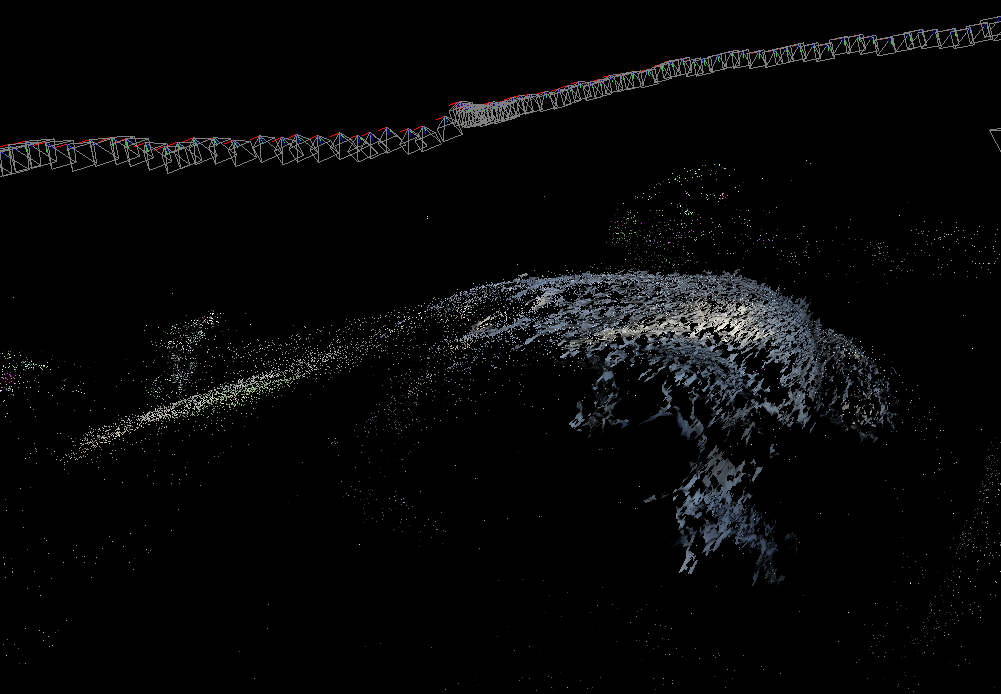
\includegraphics[width=0.5\linewidth]{figs/umvedense.png}
% 	\caption{%
% 	Final da reconstrução via UMVE, percebe-se que alguns pontos não foram considerados, tendo como resultado uma "nuvem de pontos" mais densa, basicamente.
% 	%\cite{Cui:Theobalt:etal:PAMI2013,Pajdla:etal:ICCV2011}.
% 	}\label{fig:UMVEdense}
% \end{figure} 

% Na reconstrução por linha de comando também é possível visualizar em qual etapa da execução o algoritmo está \ref{fig:passosMVE}, configurar alguns parâmetros e inclusive mostrar a porcentagem de progresso do comando. Foram executados os comandos declarados nesta seção.  O \emph{sfmrecon} demorou cerca de 1 minuto e meio \ref{fig:MVESfM}.

% \begin{figure}[!h]
% 	\centering
% 	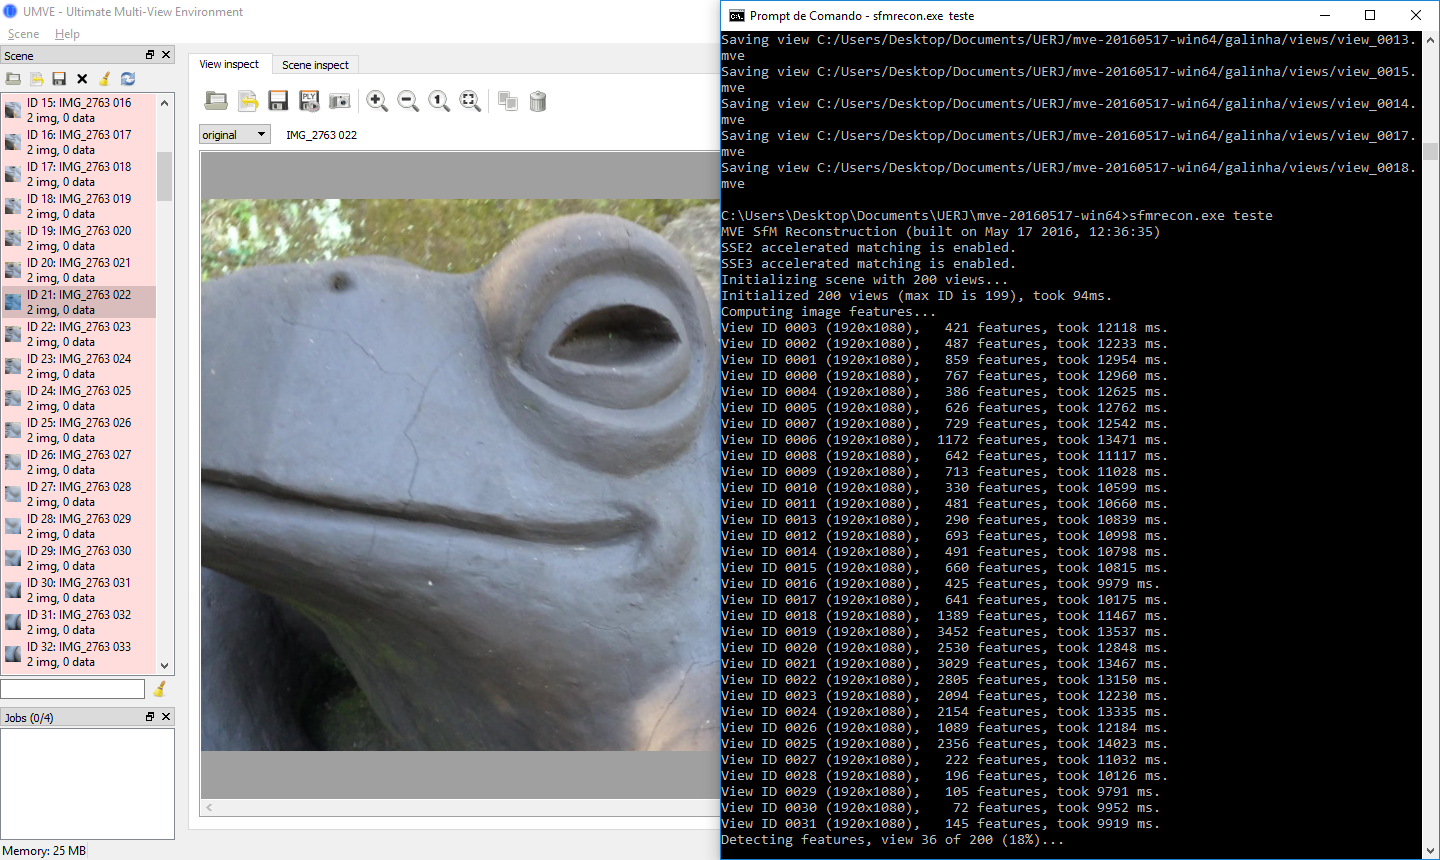
\includegraphics[width=0.5\linewidth]{figs/umve2sfm.png} (a)
% 	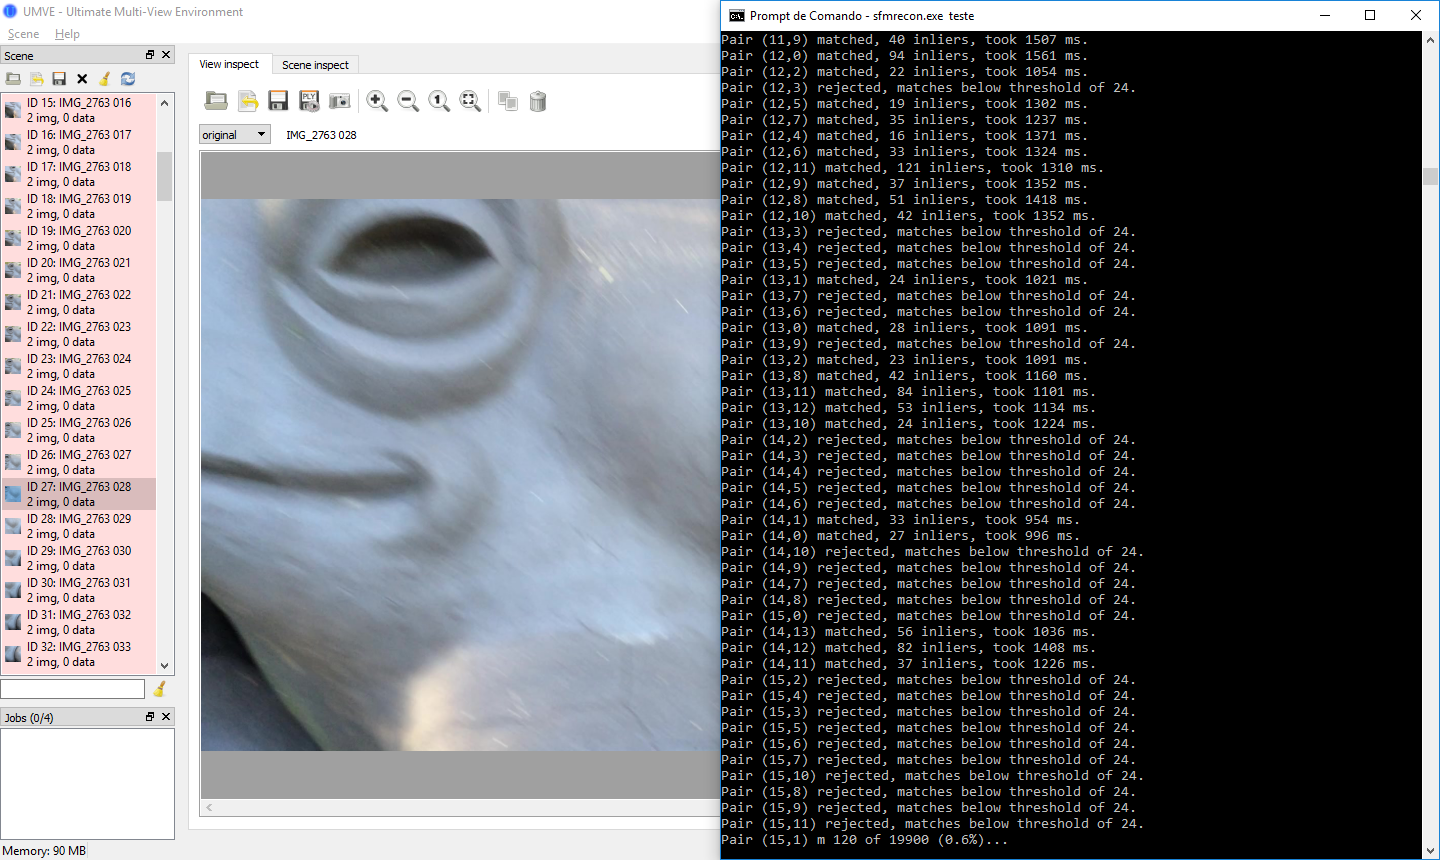
\includegraphics[width=0.5\linewidth]{figs/umve3sfmfeature.png} (b)
% 	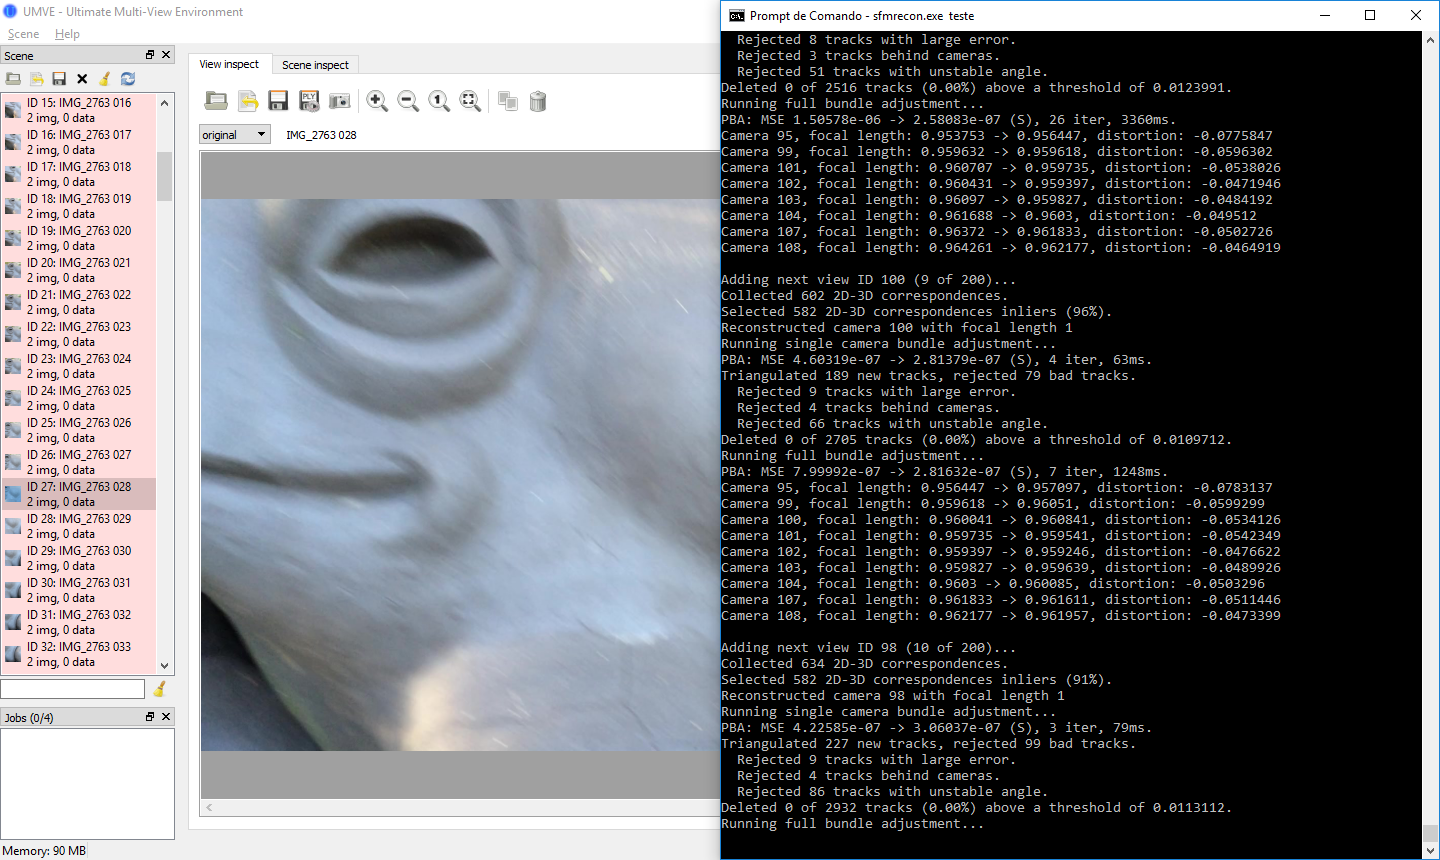
\includegraphics[width=0.5\linewidth]{figs/umve4ba.png} (c)
% 	\caption{%
% 	Processos dentro do comando \emph{sfmrecon}, onde (a) estão sendo detectadas as \emph{features} do conjunto de imagens. Em (b) está computado o \emph{pairwise matching} e em (c) está no processo de \emph{Bundle Adjustment}~\cite{bundleAdjustmentSlide}, usando condições-padrão para as câmeras.
% 	%\cite{Cui:Theobalt:etal:PAMI2013,Pajdla:etal:ICCV2011}.
% 	}\label{fig:passosMVE}
% \end{figure} 

% \begin{figure}[!h]
% 	\centering
% 	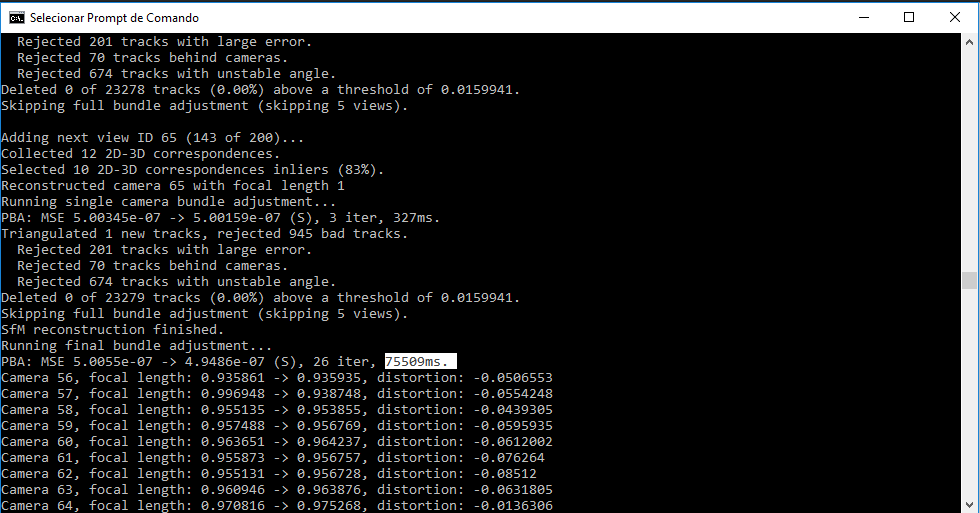
\includegraphics[width=0.8\linewidth]{figs/sfmmve.png}
% 	\caption{%
% 	Término do comando \emph{sfmrecon}, onde demorou cerca de 1 minuto e meio (75509 milisegundos).
% 	%\cite{Cui:Theobalt:etal:PAMI2013,Pajdla:etal:ICCV2011}.
% 	}\label{fig:MVESfM}
% \end{figure}

% O próximo comando, \emph{dmrecon} demorou cerca de 4 horas, usando como configuração um nível L2, com 20 vizinhos \ref{fig:MVEDenseRecon}. Usando um nível L0, o algoritmo rodou durante 6 horas aproximadamente e foi cancelado devido à demora na execução. 

% \begin{figure}[!h]
% 	\centering
% 	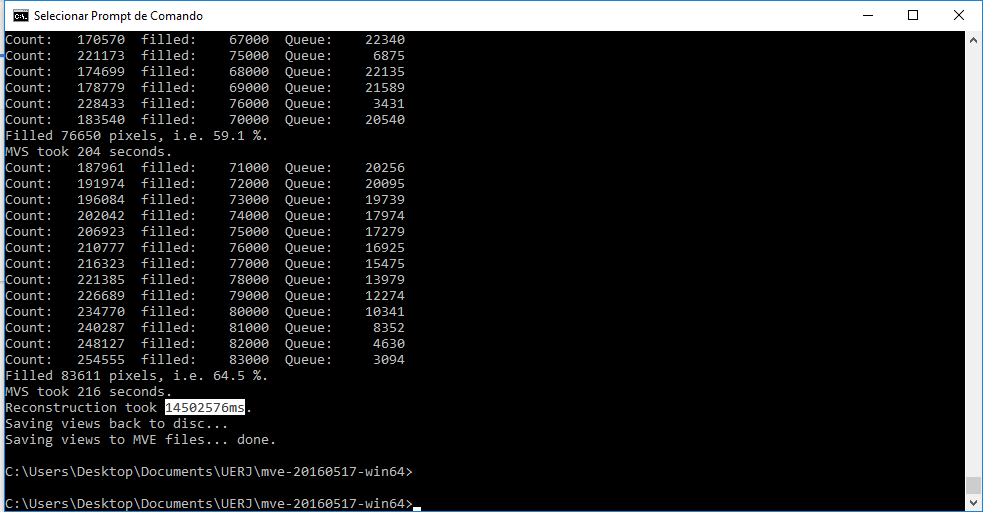
\includegraphics[width=0.8\linewidth]{figs/umvetempo.png}
% 	\caption{%
% 	Término do comando \emph{dmrecon}, onde demorou cerca de 4 horas (14502576 milisegundos).
% 	%\cite{Cui:Theobalt:etal:PAMI2013,Pajdla:etal:ICCV2011}.
% 	}\label{fig:MVEDenseRecon}
% \end{figure} 

% Usando o \emph{scene2pet}, é necessário em qual nível estamos reconstruindo e também uma saída válida. Por exemplo: "scene2pset.exe -Fnivel cena output". Onde o nível poderá ser um 0 (-F0), 1 (-F1) e assim por diante, a cena é o \emph{input} e o \emph{output} é um arquivo de extensão configurável, neste caso \emph{.ply} \ref{fig:MVEScene2Pet}. Este comando foi rápido, demorou cerca de 10 minutos, levando em conta todos os níveis.

% \begin{figure}[!h]
% 	\centering
% 	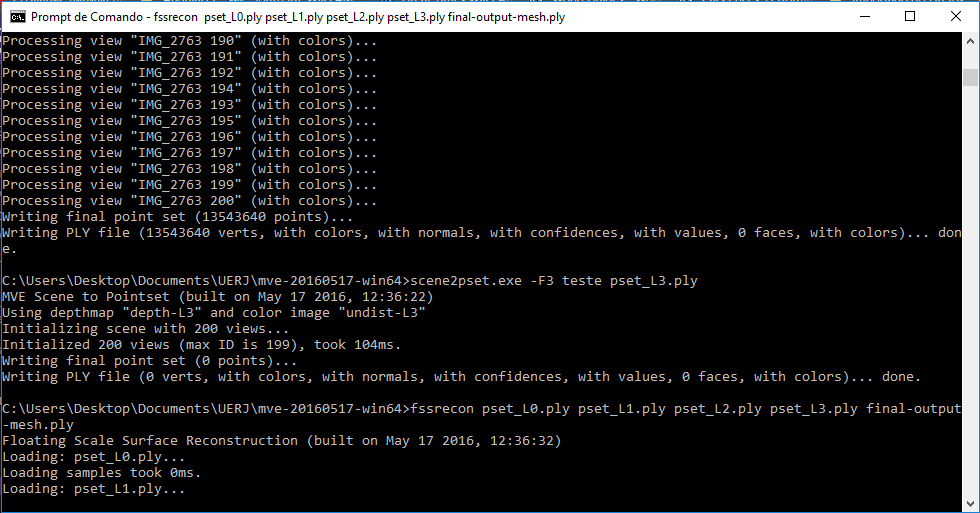
\includegraphics[width=0.8\linewidth]{figs/mvemesh.png}
% 	\caption{%
% 	Execução dos comandos \emph{scene2pset}, nos níveis -F0, -F1, -F2 e -F3.
% 	%\cite{Cui:Theobalt:etal:PAMI2013,Pajdla:etal:ICCV2011}.
% 	}\label{fig:MVEscene2pset}
% \end{figure} 

% Para juntar todos os níveis do \emph{scene2pset}, foi usado o \emph{fssrecon}, que gera uma única reconstrução. Este processo demorou bastante, cerca de 7 horas \ref{fig:MVEFSSR}. Que teve como resultado a malha \ref{fig:MVEFSSRMesh}.

% \begin{figure}[!h]
% 	\centering
% 	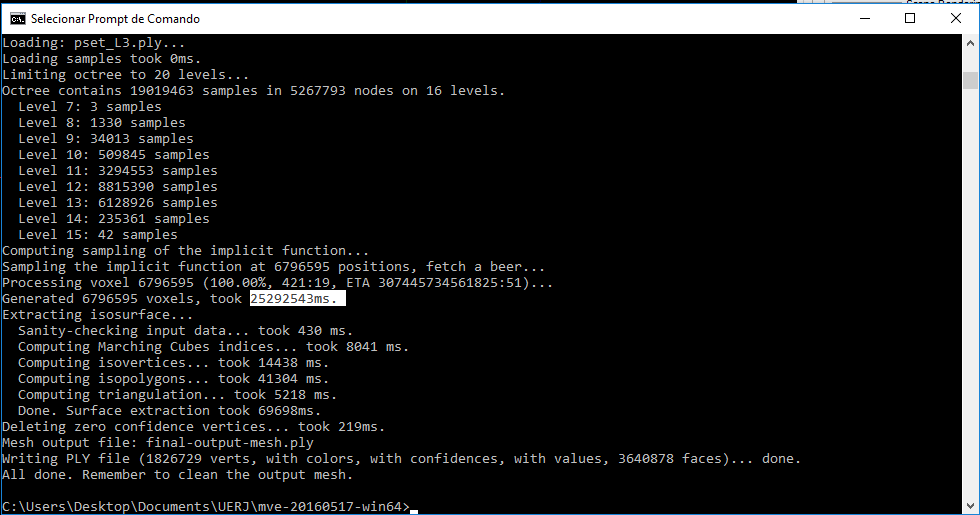
\includegraphics[width=0.8\linewidth]{figs/mvemeshtempo2.png}
% 	\caption{%
% 	Progressão do comando \emph{fssrecon}, onde possui o ETA -- \emph{Estimated Time of Arrival}.
% 	%\cite{Cui:Theobalt:etal:PAMI2013,Pajdla:etal:ICCV2011}.
% 	}\label{fig:MVEFSSR}
% \end{figure} 

% \begin{figure}[!h]
% 	\centering
% 	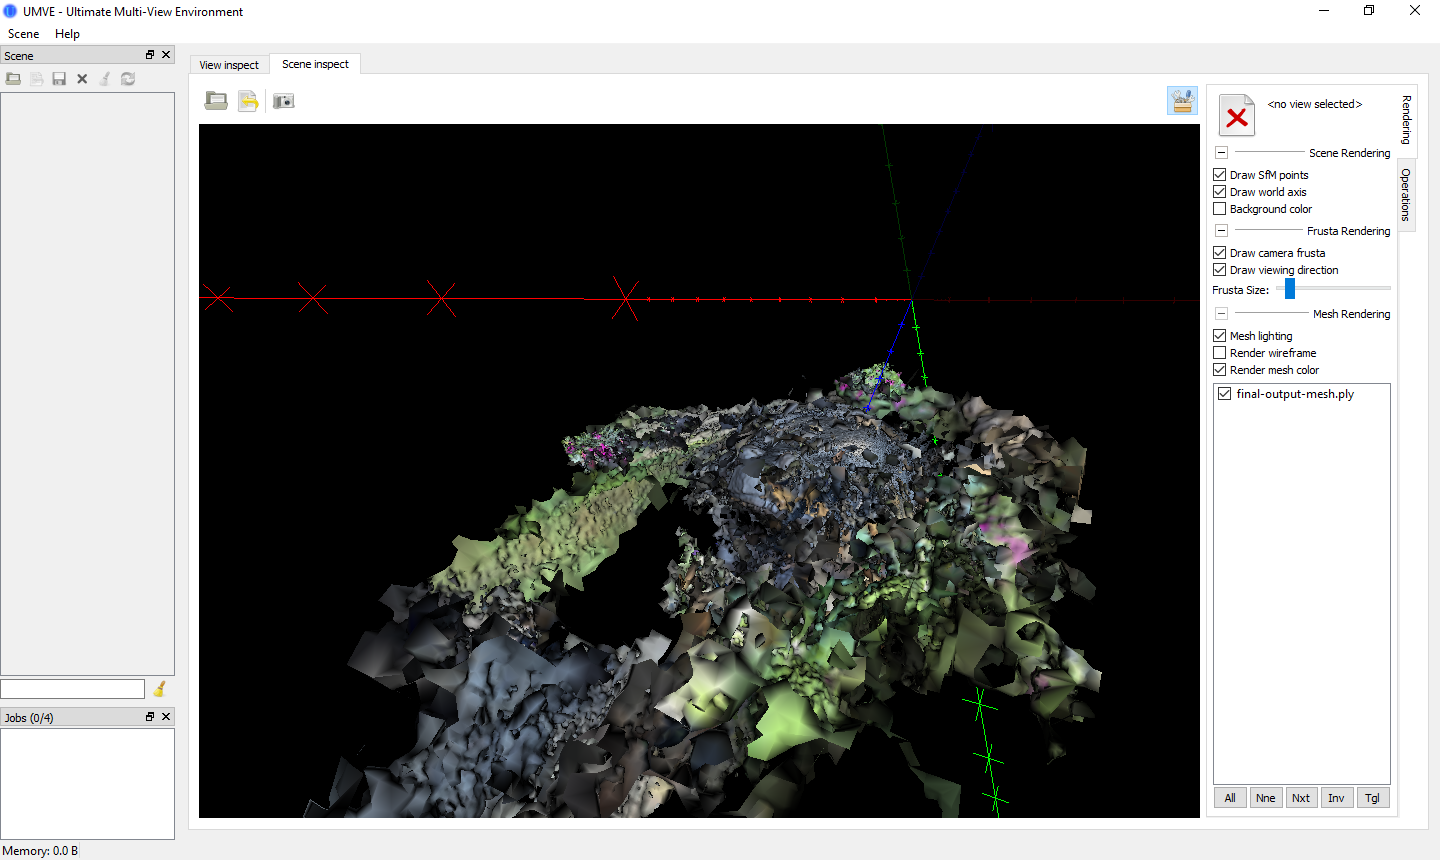
\includegraphics[width=1\linewidth]{figs/mvemeshout.png}
% 	\caption{%
% 	Malha com ruídos proveniente do comando \emph{fssrecon}.
% 	%\cite{Cui:Theobalt:etal:PAMI2013,Pajdla:etal:ICCV2011}.
% 	}\label{fig:MVEFSSRMesh}
% \end{figure} 

% Finalmente, basta limpar a malha atual com o comando \emph{meshclean}, onde foi obtido o resultado \ref{MVEMeshClean}.

% \begin{figure}[!h]
% 	\centering
% 	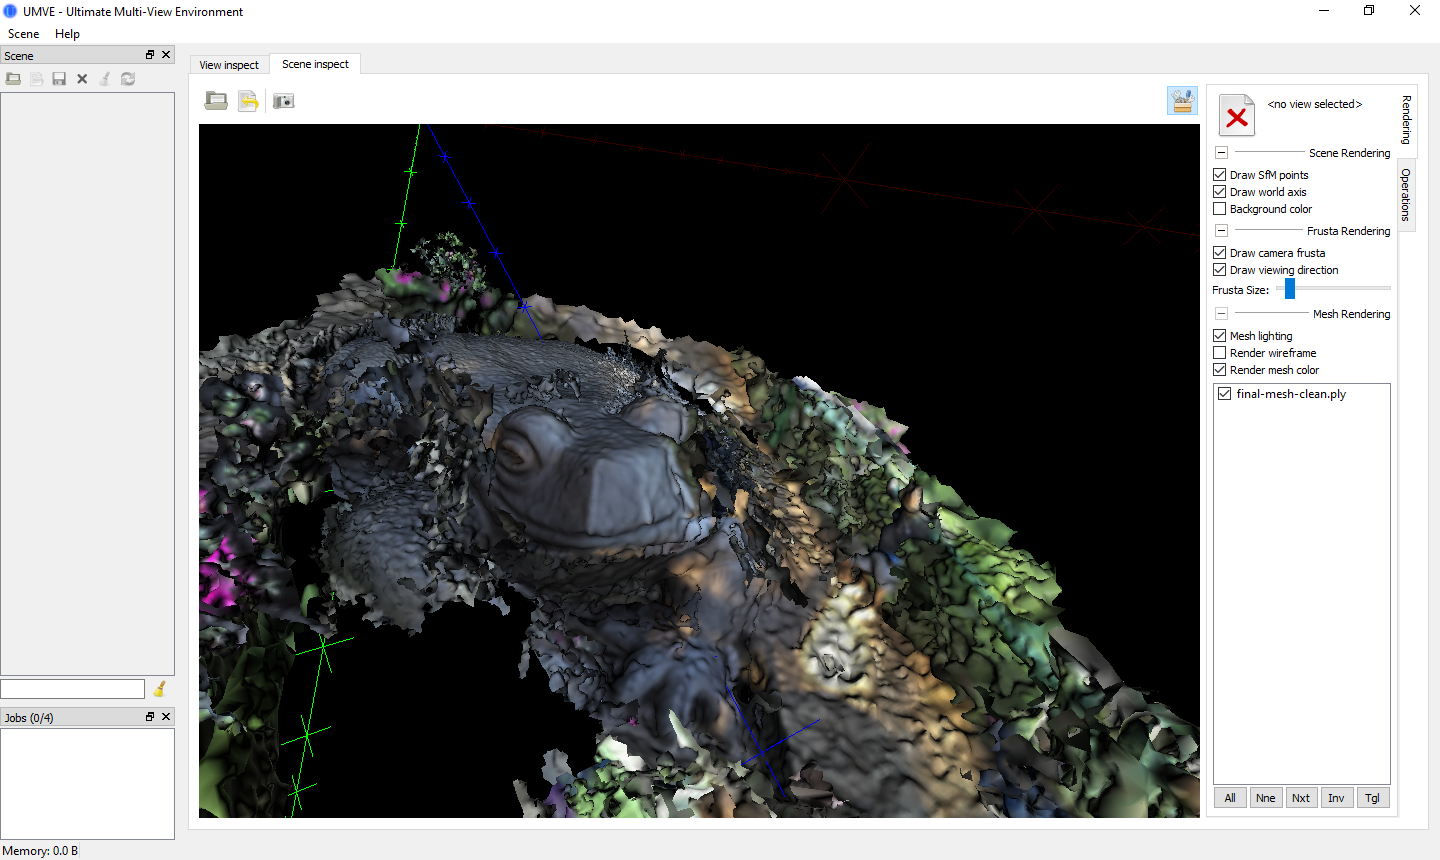
\includegraphics[width=1\linewidth]{figs/mvemeshclean.png}
% 	\caption{%
% 	Resultado final, após a remoção dos ruídos da malha.
% 	%\cite{Cui:Theobalt:etal:PAMI2013,Pajdla:etal:ICCV2011}.
% 	}\label{fig:MVEMeshClean}
% \end{figure} 

\section{VisualSfM}\label{sec:visualsfm}
%======================================================================================
%
\subsection*{Introdução}

VisualSfM~\cite{wu2011visualsfm} é um \emph{software} baseado em fotogrametria que faz todo o processo de reconstrução 3D de um objeto e que pode ser usado por linha de comando ou então pela interface gráfica, que é ótima, por sinal. É altamente customizável, podemos utilizar o CUDA da NVIDIA, ou OpenGL, especificar a lista de pares para correspondência de imagens, usar detectores de \emph{features} próprios, velocidade da detecção de \emph{features}, da reconstrução densa, dentre outros parâmetros. Ou seja, é um \emph{software} robusto, que pode ser usado em Linux, Windows ou até mesmo Mac.

Além disso, o VisualSfM é capaz de mostrar a matriz de correspondência de \emph{features}, número de \emph{features}, rodar um \emph{Bundle Adjustment} independente, usar um Level 0 no PVMS, alterar a memória de GPU usada na reconstrução, deletar uma reconstrução indesejável ou até mesmo alterar parâmetros.

\subsection*{Procedimento}

Sua linha de reconstrução é parecida com o MVE~\ref{sec:mve}, porém é mais intuitiva. Em sua interface, possui um Log de mensagens e erros que por ventura venham a acontecer e na parte de cima, alguns botões \ref{fig:pipelineVisualSfM}

\begin{figure}[!h]
	\centering
	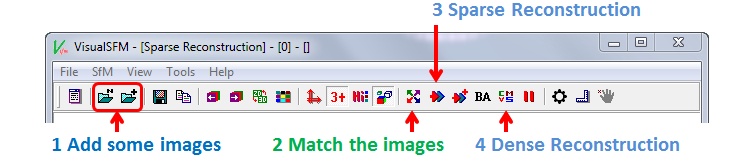
\includegraphics[width=1\linewidth]{figs/pipelinevisualsfm.png}
	\caption{%
	Botões na parte superior da interface gráfica, este seria o procedimento padrão de funcionamento do \emph{software}.
	\protect\cite{wu2011visualsfm}
	}\label{fig:pipelineVisualSfM}
\end{figure}

Como demonstrado na imagem \ref{fig:pipelineVisualSfM}, o funcionamento seria da seguinte forma:

\begin{itemize}
\item \textbf{1 - Adicionar algumas imagens.} Este é o primeiro passo, para começar uma reconstrução, primeiro adiciona-se imagens ao \emph{software}, pode ser uma única foto, um conjunto de fotos, incrementar o conjunto já existente ou então abrir um arquivo de extensão .nvm, que é interpretado como uma reconstrução esparsa previamente feita.

\item \textbf{2 - Correspondência de imagens.} Agora, o \emph{software} roda o algoritmo SIFT, realizando todas as correspondências entre os \emph{features}, que já foi discutido anteriormente.

\item \textbf{3 - Reconstrução esparsa.} Neste passo, o VisualSfM roda o algoritmo de reconstrução esparsa (PBA/MCBA)~\cite{wu2011multicore} em todos os \emph{features} descobertos no passo passado. 


PBA/MCBA -- \emph{Multi-Core Bundle Adjustment}\label{pba}

\emph{Bundle} refere-se aos feixes de luz que refletem em cada \emph{feature} 3D e vão para o centro de cada câmera da cena a ser reconstruída. Com isso, o \emph{Bundle Adjustment} é o problema de refinar uma reconstrução visual para produzir estimativas com a visualização de parâmetros (estimativa e/ou calibração de câmeras), juntamente com as estruturas 3D.

Solucionadores de problemas de \emph{Bundle Adjustment}~\cite{bundleAdjustmentSlide} resumem-se em minimizar o erro de reprojeção \ref{fig:bundleAdjustment} entre as posições de imagem dos pontos de imagem observados e previstos, o que é expresso como a soma de quadrados de um grande número de funções não-lineares de valor real. Assim, a minimização é obtida usando algoritmos de mínimos quadrados não-lineares. Destes, Levenberg-Marquardt~\cite{more1978levenberg} provou ser um dos mais bem sucedidos devido à sua facilidade de implementação e ao uso de uma estratégia de amortecimento eficaz que lhe confere a capacidade de convergir rapidamente de uma ampla gama de suposições iniciais. Ao linearizar iterativamente a função a ser minimizada na vizinhança da estimativa atual, o algoritmo de Levenberg-Marquardt envolve a solução de sistemas lineares denominados equações normais. Ao resolver os problemas de minimização que surgem na estrutura do \emph{Bundle Adjustment}, as equações normais tem uma estrutura de bloco esparsa devido à falta de interação entre os parâmetros para diferentes pontos 3D e câmeras. Isso pode ser explorado para obter enormes benefícios computacionais ao empregar uma variante esparsa do algoritmo de Levenberg-Marquardt que aproveita explicitamente o padrão de zeros de equações normais, evitando armazenar e operar em elementos zero.

\begin{figure}[!h]
	\centering
	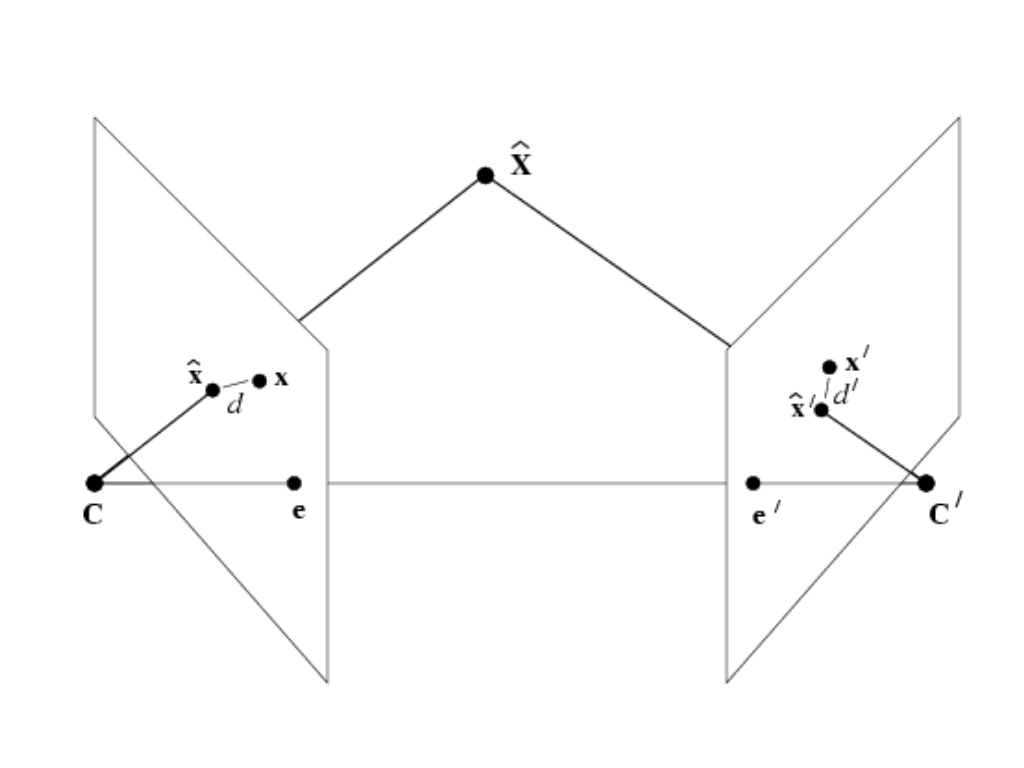
\includegraphics[width=0.5\linewidth]{figs/bundleAdjustment.png}
	\caption{
	Dado um ponto de um objeto 3D $\widehat{X}$, sua reprojeção nas câmeras $C$ e $C'$, são, respectivamente, $x$ e $x'$. Esses pontos possuem um erro de reprojeção $d$ e $d'$ e ao utilizar o PBA/MCBA, os pontos $x$ e $x'$ serão reajustados como $\widehat{x}$ e $\widehat{x'}$, respectivamente. 
	\protect\cite{3DCompVision2Didier}
	}\label{fig:bundleAdjustment}
\end{figure}

Neste caso, o PBA/MCBA~\cite{furukawa2009accurate,wu2011multicore} é um algoritmo que utiliza, de forma eficiente, os núcleos do computador, sendo até 10 vezes mais rápido, em CPU e 30 vezes, em GPU, em comparação ao utilizado na conferência ECCV de 2010. É o primeiro sistema publicado, baseado em GPU que escala com maiores problemas de Bundle Adjustments. Isto abriu a porta para resolver problemas ainda maiores. Ele funciona observando o passo inexato de resolução não-linear usando Levenberg Mardquardt, que pode ser implementado sem armazenar nenhuma matriz (Hessiana, complemento de Schur ou Jacobiana) na memória. Para sistemas de núcleo único isso se traduzia em memória de troca por tempo, mas em GPUs, isso leva a um surpreendente ganho, no espaço e no tempo. Outra surpresa é que a aritmética de precisão única, quando combinada com técnicas de normalização adequadas, dá resultados comparáveis aos obtidos por um solucionador de problemas usando aritmética de dupla precisão. Isso resulta em mais espaço e economia de tempo.

Este algoritmo recebe como entrada conjunto de localizações e correspondências de \emph{features} de imagens, o objetivo do \emph{Bundle Adjustment} é encontrar posições de 3 pontos e parâmetros de câmera que minimizem o erro de reprojeção. Esse problema de otimização geralmente é formulado como um problema de mínimos quadrados não-lineares, onde o erro é a norma L2 quadrada da diferença entre a localização da característica observada e a projeção do ponto 3D correspondente no plano da imagem da câmera.

Assumindo que $x$ é um vetor de parâmetros e $f(x) = [f1(x), \dots, f_k(x)]$ é o vetor de erros de projeção de uma reconstrução 3D. O problema de otimização pode ser  formulado como um problema de mínimos quadrados não-linear:

\begin{equation}
x^* = \text{argmin}_x \sum_{i=1}^k || f_i(x)||^2
\end{equation}

O algoritmo de Levenberg-Marquardt (LM) é o mais conhecido para resolução de problemas de mínimos quadrados não-lineares. O LM funciona resolvendo uma série de aproximações lineares regularizadas ao problema não-linear original. Seja $J(x)$ a Jacobiana de $f(x)$, então em cada iteração LM resolve um problema linear de mínimos quadrados da forma:

\begin{equation}
\label{eq:LM}
\delta* = \text{argmin}_\delta || J(x)\delta + f(x) ||^2 + \lambda ||D(x)\delta||^2 
\end{equation}
e, atualiza $x$, da forma:

\begin{algorithm}
\label{LMattX}
\begin{algorithmic}[1]
\State $\text{caso} (||f(x + \delta^*)|| < || f(x) ||)$
\State	$x = x + \delta^*$
\end{algorithmic}
\end{algorithm}

%\begin{algorithmic}[1]
%\BState $\text{caso} (||f(x + \delta^*)|| \le || f(x) ||)$
%\State	$x = x + \delta^*$
%\end{algorithmic}

Aqui, $D(x)$ é uma matriz diagonal não-negativa, tipicamente a raíz quadrada da diagonal da matriz $J(x)^T J(x)$ e $\lambda$ são parâmetros não-negativos que controlam a limite da regularização, que, por sua vez, é necessária para garantir um algoritmo convergente. O LM atualiza o valor de $\lambda$ a cada passo, baseado no quanto a Jacobiana ($J(x)$) está próxima da função original ($f(x)$).
Resolver \ref{eq:LM} é equivalente à resolver as equacões normais
\begin{equation}
\label{eq:LMNormal}
(J^T J + \lambda D^T D)\delta = -J^T f
\end{equation}
onde retiramos a dependência de $x$. A matriz $H_\lambda = J^T J + \lambda D^T D$ é conhecida como a matriz Hessiana aumentada. 

No \emph{Bundle Adjustment}, o parâmetro "vetor" é tipicamente organizado como $x = [x_c;x_p]$, onde $x_c$ é o vetor de parâmetros da câmera e $x_p$ é o vetor de parâmetros do ponto. Similarmente para $D$, $\delta$ e $J$, usaremos subscritos $c$ e $p$ para denotar parâmetros da câmera e do ponto, respectivamente. 
Seja $U = J_c^T J_c$, $V = J_p^T J_p$, $U_lambda = U + \lambda D_c^T D_c$, $V_\lambda = V + \lambda D_p^T D_p$ e $W = J_c^T J_p$, então \ref{eq:LMNormal} pode ser re-escrita como um bloco de sistema linear estruturado

\[
\begin{bmatrix}
U_\lambda & W \\
W^T & V_\lambda 
\end{bmatrix}
\begin{bmatrix}
\delta_c\\ 
\delta_p
\end{bmatrix} =
-\begin{bmatrix}
J_c^T f\\ 
J_p^T f
\end{bmatrix}
\]

Vale ressaltar que, para a maioria dos problemas de \emph{Bundle Adjustment}, $U_\lambda$ e $V_\lambda$ são matrizes diagonais de blocos. Esta observação está no fundamento do truque do complemento de Schur usado para resolver esse sistema linear de forma eficiente, onde, ao aplicar a eliminação Gaussiana nos parâmetros do ponto, obtemos um sistema linear consistindo apenas nos parâmetros da câmera:

\begin{equation}
\label{eq:SchurComplementar}
(U_\lambda - W V_\lambda^-1 W^T)\delta_c = -J_c^T f + WV_\lambda^-1 J_p^T f
\end{equation}

Onde $S = U_\lambda - W V_\lambda^-1 W^T$ é o complemento de Schur ou a matriz reduzida da câmera. Com a solução para \ref{eq:SchurComplementar}, conseguimos obter os parâmetros do ponto com substituição regressiva:

\begin{equation}
\delta_p = -V_\lambda^-1(J_p^T f + W^T \delta_c)
\end{equation}

Caso S for simétrica positiva-definida, a fatorização de Cholesky é indicado para a resolução de \ref{eq:SchurComplementar}. 

No caso do MCBA, ele combina o uso de algoritmos de gradientes de conjugados pré-condicionados e algoritmos inexatos LM para resolução dessas equações  com alguns pré-condicionadores simples e computacionalmente baratos. 

combinando um algoritmo Inexact Step LM e gradientes de conjugado pré-condicionado com alguns pré-condicionadores simples e computacionalmente baratos. O

O algoritmo MCBA, une o paralelismo da GPU e técnicas de uso de multi-núcleos da GPU e a combinação  de algoritmos de gradientes de conjugados pré-condicionados e algoritmos inexatos LM para resolução dessas equações  com alguns pré-condicionadores simples e computacionalmente baratos. 


% Abordagem geral [editar]
% O ajuste do pacote resume-se a minimizar o erro de reprojecção entre as posições de imagem dos pontos de imagem observados e previstos, o que é expresso como a soma de quadrados de um grande número de funções não-lineares de valor real. Assim, a minimização é conseguida usando algoritmos de mínimos quadrados não-lineares. Destes, Levenberg-Marquardt provou ser um dos mais bem sucedidos devido à sua facilidade de implementação e ao uso de uma estratégia de amortecimento eficaz que lhe confere a capacidade de convergir rapidamente de uma ampla gama de suposições iniciais. Ao linearizar iterativamente a função a ser minimizada na vizinhança da estimativa atual, o algoritmo de Levenberg-Marquardt envolve a solução de sistemas lineares denominados equações normais. Ao resolver os problemas de minimização que surgem na estrutura do ajuste do feixe, as equações normais têm uma estrutura de bloco esparsa devido à falta de interação entre os parâmetros para diferentes pontos 3D e câmeras. Isso pode ser explorado para obter enormes benefícios computacionais ao empregar uma variante esparsa do algoritmo de Levenberg-Marquardt que aproveita explicitamente o padrão de zeros de equações normais, evitando armazenar e operar em elementos zero. [2]: 3










%------------------------------------------------------------------------------------%

% Nos últimos anos, a paralelização baseada em GPU atraiu muita atenção para a pesquisa. Isso inclui o propósito geral
% bibliotecas como nVidia's Sparse Matrix-Vector Multiplication
% [3] e o trabalho de Li e Saad em várias GPUs baseadas em GPU
% algoritmos e técnicas de pré-condicionamento [10]. Embora seja
% Você pode criar um sistema de ajuste de pacotes usando estes
% bibliotecas de propósito geral, melhor desempenho é alcançado por
% construindo um sistema que explora a estrutura do problema
% tanto quanto possível.
% No campo da visão computacional, muitos algoritmos têm
% foi portado para a GPU com ganhos de velocidade significativos. Este
% inclui detecção de recursos, combinação de recursos e reconstrução estéreo,
% etc. Uma demonstração impressionante é o multiGPU
% sistema descrito em [6]. Vale a pena
% observando, no entanto, que o passo de ajuste do feixe neste sistema
% ainda foi realizada usando CPUs de um único segmento.
% Dado os constrangimentos do modelo de programação GPU,
% não é trivial obter algoritmos de ajuste de pacote para executar
% em GPUs. Recentemente, Gupta et al [8] tomaram uma abordagem híbrida
% para executar cálculos de sobreposição em GPU e CPU,
% onde as matrizes de Hessian e complementos de Schur são
% construído em GPU. Isso não é prático para grandes problemas
% (milhares de imagens ou mais), especialmente para a comunidade
% Coleções de fotos com complementos densos de Schur.
% Mesmo as GPUs de estação de trabalho da próxima geração têm uma pequena quantidade
% para armazenar os complementos Schur (mesmo o Hessian
% matronas ou jacobios), pode não ser viável. Até
% com memória suficiente, a construção de complementos de Schur
% ainda seria muito caro para grandes problemas.
% O PBA é um algoritmo utilizado para minimizar o erro geométrico proveniente da reprojeção de cada \emph{feature} da etapa de triangulação. Implementado em GPU (Graphic Processor Unit) para computar a Distância de Transformação Euclidiana (EDT -- Euclidean Distance Transform) para uma imagem binária em 2D ou em dimensões superiores. Particionando a imagem em pequenas bandas, para serem processadas e, posteriormente, juntando-as simultaneamente, o PBA calcula o EDT exato com ótimo trabalho linear total, alto nível de paralelismo e um bom padrão de acesso à memória. Este algoritmo foi um dos precursores ao tentar explorar o máximo desempenho da GPU no cálculo da EDT exata. 


% O PBA é divido em 3 fases:

% \begin{itemize}
% \item Band Sweeping
% \item Hierarchical Merging
% \item Block coloring
% \end{itemize}

% Band Sweeping

% In this phase, for each row, we want to compute the 1D Voronoi
% diagram using only those sites in the same row. A trivial approach
% would be to use a two-pass sweeping (left to right and then right to
% left sweeping), similar to SKW [Schneider et al. 2009]. This, however,
% restricts the parallelism to only one thread per row, potentially
% under-utilizing the GPU. One could also use a 1D JFA [Rong and
% Tan 2007] with better utilization of the GPU at the cost of higher
% total work. Another possibility would be to use a method similar
% to the work efficient parallel prefix sum [Harris et al. 2007]. This
% approach is too complicated as compared to our following simple,
% yet work and time efficient approach.
% Our approach extends the na¨ıve two-pass sweeping approach, with
% the introduction of bands to effectively increase the level of parallelism.
% First, we divide the input image into m1 vertical bands
% of equal size, and use one thread to handle one row in each band,
% performing the left-right sweeps. Next, for one site to propagate
% its information to a different band (on the same row), it has to be
% the closest site to the first or the last pixel of its band. As such, to
% combine the result of different bands into the needed answer, we
% first propagate the information among the first and the last pixels
% of all bands using a parallel prefix approach on these 2m1 pixels.
% With this, the first and the last pixel of each band have the correct
% information, whereas other pixels inside a band can then obtain the
% correct closest sites by updating (if needed) their current information
% with that of the first and the last pixel of their band. This can
% be done in parallel in constant time using N threads.

% Hierarchical Merging

\item \textbf{4 - Reconstrução densa.} Finalmente, acaba a reconstrução rodando o algoritmo de reconstrução densa~\cite{gavadense} CMVS/PMVS-2 embutido no próprio VisualSfM.

%FALAR SOBRE O ALGORITMO DE RECONSTRUCAO DENSA == PMVS-2/CMVS%
CMVS/PMVS-2 (\emph{Clustering Views for Multi-view Stereo / Patch-based for Multi-view Stereo version 2})

%Um dos algoritmos mais utilizados Furukawa o CMVS que possui o PMVS-2 (Patch-based Multi-view Stereo versão 2) implementado dentro dele. O PMVS-2 é uma abordagem automatizada para reconstruções densas de superfícies, baseada em combinações de features de imagens múltiplas e técnicas de correspondência baseadas em áreas, com imagens calibradas.
%Ele utiliza conjuntos de imagens e parâmetros de câmera, então reconstrói a estrutura 3D de um objeto, ou a cena visível nas imagens. Um ponto positivo deste \emph{software} é que ele só reconstrói estruturas rígidas, ou seja, ele ignora automaticamente objetos não rígidos como pessoas na frente de uma construção ou escultura, por exemplo. A saída do \emph{software} é um conjunto orientado de pontos ao invés de um modelo poligonal (ou malha), onde tanto a coordenada 3D quanto a superfície normal são estimados em cada ponto orientado.

Muitos algoritmos Multi-View Stereo (MVS) não escalam tão bem com um grande número de imagens de entrada ou em uma alta resolução, pois necessitam de muita memória e recursos computacionais. A palavra-chave do CMVS~\cite{visualSfMPMVS,wu2013towards,li2013improving} é escalabilidade, pois seu propósito é utilizar imagens provenientes de sites na internet, em diferentes resoluções, como o Flickr.com.  
Ele usa a saída do Structure from Motion -- SfM (mais especificamente a saída do passo anterior, do PBA) e utiliza como entrada. Após isso, decompõe as imagens de entrada como um conjunto de \emph{clusters} de imagens com tamanhos gerenciáveis. O MVS pode ser usado para processar cada \emph{cluster} de forma independente e em paralelo, onde a união das reconstruções de todos os \emph{clusters} não deve perder detalhes que poderiam ser obtidos através do conjunto de imagens.

A formulação dos \emph{clusters} é projetada para satisfazer três restrições: 
\begin{itemize}
\item{(1) as imagens redundantes são excluídas dos \emph{clusters} (compacidade)}
\item{(2) cada \emph{cluster} é pequeno o suficiente para uma reconstrução MVS (restrição de tamanho)}
\item{(3) as reconstruções MVS destes \emph{clusters} resultam em uma perda mínima de conteúdo e detalhes em comparação com o que pode ser obtido através do processamento do conjunto completo de imagens (cobertura).}
\end{itemize}

A compacidade é importante para a eficiência computacional, mas também para melhorar precisão, pois as coleções de fotos da Internet geralmente contêm centenas ou milhares de fotos adquiridas de quase mesmo ponto de vista, ou seja, um conjunto composto inteiramente informações duplicadas.

Em outras palavras, a sobreposição de \emph{clusters} é definida por:

\begin{itemize}
\item Minimizar $\sum_{k} |C_k|$ (compacidade)
\item $\forall k |C_k| \le \alpha$, onde $\alpha$ é determinado por recursos computacionais, principalmente por limitações de memória. (tamanho)
\item $\forall i \frac{\text{ \# pontos cobertos em } I_i}{\text{ \# pontos em } I_i} \ge \delta$, onde $\delta$ é uma constante de proporção de pontos cobertos. (cobertura)
\end{itemize}

O CMVS pode ser resumido em quatro passos:

\begin{itemize}
\item Filtro SFM -- agrupamento de pontos SFM
\item Seleção de imagens -- remove imagens reduntantes
\item Divisão de \emph{cluster} -- reforça a restrição de tamanho
\item Adição de imagens -- reforça a cobertura
\end{itemize}

\subsubsection{Filtro SFM}
A obtenção de medidas precisas de visibilidade de pontos é fundamental para o sucesso do procedimento de visualização baseado em \emph{clusters}. Os recursos da imagem não detectados ou incomparáveis levam a erros nas estimativas de visibilidade do ponto $V_j$ (geralmente na forma de imagens que estão faltando). Obtemos estimativas de visibilidade mais confiáveis ao agregar dados da visibilidade em uma vizinhança local, e mesclando os pontos nessa vizinhança. A posição do ponto mesclado é a média de seus vizinhos, enquanto a visibilidade se torna a união. Este passo também reduz significativamente o número de pontos SFM e melhora o tempo de execução das tres etapas restantes. Especificamente, a partir de um conjunto de pontos SFM, um ponto é selecionado, combinado com seus vizinhos (mesclado) e, este ponto mesclado é emitido, após isso, o ponto original e seus vizinhos são removidos do conjunto de entrada. Esse procedimento é repetido até o conjunto de entrada estar vazio. O conjunto de pontos mesclados torna-se o novo conjunto de pontos, que, pode ser denotado por ${P_j}^2$. %figura 4%

\subsubsection{Seleção de imagens}
Começando com o conjunto completo de imagens, cada imagem é testada e removida se a restrição de cobertura ainda for realizada após a remoção. O teste de remoção é realizado para todas as imagens enumeradas em ordem crescente de resolução de imagem (\# de pixels), de modo que as imagens de baixa resolução sejam removidas primeiro. Observe que as imagens são descartadas permanentemente nesta etapa para acelerar as seguintes etapas principais de otimização.

\subsection{Divisão de \emph{cluster}}
Em seguida, é aplicada a restrição de tamanho dividindo os \emph{clusters}, ignorando a cobertura. Mais especificamente, um \emph{cluster} de imagens é dividido em componentes menores caso viole a restrição de tamanho. A divisão de um \emph{cluster} é realizada pelo algoritmo \emph{Normalized-Cuts} %CITAR#
[23] em um gráfico de visibilidade, onde os nós são imagens. O peso dA borda entre um par de imagens ($I_l, I_m$) mede o quanto a $I_l$ e $I_m$ contribuem, juntos,  para a reconstrução MVS em pontos SFM relevantes: 

$e_{lm} = \sum_{P_j \in \Theta ^{lm}} \frac{f(Pj,{Il, Im})}{f(Pj, Vj )}$, onde $\Theta ^{lm}$ denota um conjunto de pontos SFM visíveis em $L_l$ e $I_m$. Intuitivamente, as imagens com alta contribuição no MVS têm pesos altos entre eles e são menos propensos a serem cortados. A divisão de um \emph{cluster} se repete até que a restrição de tamanho seja satisfeita para todos os \emph{clusters}.

\subsubsection{Adição de imagens}
A restrição de cobertura pode ter sido violada na etapa anterior, e agora são adicionadas imagens a cada \emph{cluster} para cobrir mais pontos SFM e restabelecer a cobertura. Nesta etapa, primeiro é construída uma lista de ações possíveis, onde cada ação mede a eficácia de adicionar uma imagem a um \emph{cluster} para aumentar a cobertura. Para cada ponto SFM que está descoberto, $P_j$, deixe $C_k = argmax_{Cl} f(Pj, Cl)$ ser o \emph{cluster} com a máxima precisão de reconstrução. 
Então, para $P_j$, é criada uma ação ${(I \rightarrow C_k), g}$ que adiciona a imagem $I (\in V_j, \not\in C_k)$ a $C_k$, onde $g$ mede a eficácia. Só são consideradas ações que adicionam imagens ao $C_k$ em vez de cada \emph{cluster} que poderia cobrir $P_j$, para eficiência computacional. Uma vez que as ações com a mesma imagem e com o mesmo \emph{cluster} são geradas a partir de vários pontos SFM, ocorre uma mescla dessas ações ao resumir a eficácia medida $g$. As ações na lista são classificadas em uma ordem decrescente de sua eficácia. Tendo construído uma lista de ações, uma abordagem seria tomar a ação com a pontuação mais alta, então refazer a lista novamente, o que é computacionalmente muito caro. 

%O objetivo é minimizar o número total de imagens $\Sigma_k |C_k|$ nos \emph{clusters} de saída, sujeito às restrições: um limite superior no tamanho de cada \emph{cluster} para que um algoritmo MVS possa ser usado para cada \emph{cluster}, independentemente: $\forall k, |C_k| ≤ \alpha$. $\alpha$ é determinado por recursos computacionais, principalmente por limitações de memória. 
%O segundo aborda a cobertura das reconstruções MVS finais. Dizemos que um ponto SFM $P_j$ é coberto se for suficientemente reconstruído pelas câmeras em pelo menos um \emph{cluster} $C_k$. Para quantificar esta noção de "bem-construído", apresentamos uma função $f(P, C)$ que mede a precisão de reconstrução esperada alcançada em uma localização 3D $P$ por um conjunto de imagens $C$. Esta função depende dos parâmetros da câmera e das taxas de amostragem de pixels, esta função é abordada em %CITAR CMVS%. 
%Dizemos que $P_j$ está coberto se a precisão da reconstrução em pelo menos um dos \emph{clusters} $C_k$ é pelo menos $\lambda$ vezes $f (Pj, Vj)$, o que é a precisão esperada obtida ao usar todas as imagens visíveis de $P_j$ ($V_j$): 
%$P_j$ está coberto se $\underset{k}{max} f(P_j, C_k \cap V_j) \ge \lambda f(Pj, Vj)$, onde $\lambda = 0,7$ nos testes apresentados \cite{CMVS}. A restrição de cobertura é que, para cada conjunto de pontos SFM visíveis em uma imagem, a proporção de pontos cobertos deve ser pelo menos $\delta$ (também definida em 0,7). Note-se que aplicamos essa relação de cobertura em cada imagem, em vez de toda a reconstrução, para incentivar uma boa cobertura espacial e uniformidade.

Em vez disso, consideramos ações cujas pontuações são mais de $0,7$ vezes a pontuação mais alta na lista, em seguida, repete-se a ação a partir do topo da lista. Como uma ação pode alterar a eficácia de outras ações semelhantes, depois de tomar uma ação, remove-se quaisquer conflito da lista, onde duas ações ${(I \rightarrow C), g}, {(I' \rightarrow C'), g' }$ estão em conflito se $I'$ e $I$ são vizinhos. A construção da lista e a adição da imagem são repetidas até que a restrição de cobertura seja satisfeita.

Após a adição da imagem, a restrição de tamanho pode ser violada e, neste caso, as duas últimas etapas são repetidas até que ambas as restrições sejam satisfeitas.

O passo seguinte, depois de obtido o \emph{cluster} das imagens, é empregado algum algoritmo de reconstrução MVS, neste caso, o PMVS-2 (Patch-based Multiview Stereo Versão 2)~\cite{visualSfMPMVS,Li2013,furukawa2010towards}.

\subsubsection{PMVS-2}

O PMVS-2 utiliza a técnica de DoG e cantos de Harris. O DoG é utilizado para detecção de bordas, subtraindo o resultado de dois Gaussianos com escalas diferentes \ref{DiffGaussian}. O operador de Harris emprega uma auto-correlação local para melhorar a consistência da borda, extraindo a borda e os cantos dos \emph{features} das imagens. A resposta de Harris é positiva em regiões com cantos, negativas em bordas e pequenas em regiões planas. Além disso, no PMVS-2, usando pontos de amostras das imagens como sementes, as linhas epipolares são usadas para decidir a região correspondente (dentro de uma área 2x2 pixels) em outra imagem, gerando \emph{patches} (cada uma definida com seu centro, normal e visibilidade) para atender às restrições na visibilidade, e levando à uma correspondência baseada em \emph{patches} entre imagens. A correspondência \emph{Multi-view} no PMVS-2 é baseada em \emph{patches} e depende da consistência fotográfica média de todos os pares visíveis. Um \emph{patch} é reconstruído usando maximizando o valor médioda consistência da foto e, em seguida, aceitando somente se o número de imagens visíveis for maior ou igual a três.  

A superfície do objeto é aproximada por um pequeno retângulo (o \emph{patch}).
O \emph{patch}(p) é um retângulo modelado pela posição central $c(p)$, pelo vetor normal $n(p)$, pelos eixos $x$ e $y$ e pela imagem de referência $R(p)$, onde a imagem é a que melhor representa a visibilidade do \emph{patch}. Seu tamanho é determinado por sua projeção na imagem de referência $R(p)$.

A imagem é divida em células (\emph{grid}), de $\beta$ x $\beta$ pixels (usualmente 2x2). O ideal é reconstruir um patch por célula. Quanto menor a célula, maior será a densidade na nuvem de pontos final.

O PMVS-2 pode ser dividido em algumas etapas:

\begin{itemize}
\item{Inicalização}
	\subitem{Detecção de \emph{features}}
	\subitem{Correspondência guiada}
\item{Expansão}
\item{Filtragem}
\end{itemize}

\subsubsection{Detecção de \emph{features}}

O PMVS-2 padrão utiliza o DoG em conjunto com o algoritmo de cantos de Harris, onde é criada uma linha epipolar, e todos os pontos em comum nesta linha são considerados consistentes para a reconstrução. 
Após isso cria-se o \emph{patch} onde o $c(p)$ é calculado pela triangulação dos \emph{features} detectados das imagens. A normal $n(p)$ é o cálculo da relação do vetor $c(p)$, multiplicado pela centro óptico da imagem, pelo módulo do numerador. E $R(p)$ é a imagem de referência propriamente dita. São otimizadas as orientações e posições de todos os \emph{patches}.
Com a inicialização finalizada, temos como resultado a reconstrução esparsa da escultura. No caso do VisualSfM, como a reconstrução esparsa já é feita em passos anteriores (com o PBA \ref{pba}), na realidade o PMVS-2 só é empregado para a reconstrução densa, ou seja, a inicialização não é feita pelo PMVS-2 no VisualSfM.

\subsubsection{Expansão}

Cada ponto 3D na nuvem de pontos é usado como semente para um algoritmo de expansão (aumento da região). Um \emph{patch} utilizado como semente é expandido da seguinte forma:

Um novo \emph{patch} é projetado em uma célula vizinha.
A posição é definida para a interseção do raio projetado para trás e no plano de seu patch pai, usando a mesma orientação (o vetor normal é propagado) e a mesma imagem de referência.
Novamente, são otimizadas as orientações e posições, porém, do novo \emph{patch}.	

\subsubsection{Filtragem}
É aplicada uma consistência de visibilidade global, onde os \emph{patches} que não são visíveis pelos centros ópticos das imagens, são descartados (estão dentro da superfície). Para isso, são utilizados dois filtros: filtro de qualidade e filtro de visibilidade \ref{filtropmvs}.

\begin{figure}[!h]
	\centering
	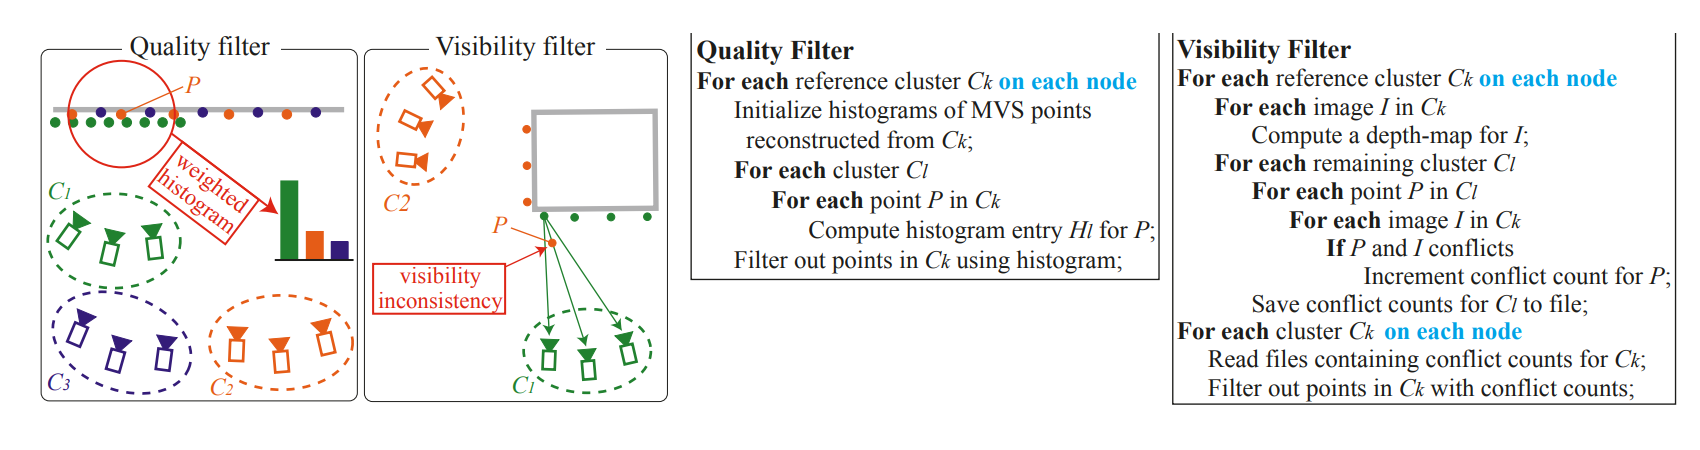
\includegraphics[width=0.5\linewidth]{figs/filtropmvs.png}
	\caption{%
	Usabilidade dos filtros de qualidade e visibilidade, onde são aplicados fora do núcleo, assim como em paralelo. À esquerda, um ponto MVS $P$ é testado usando os filtros. À direita, temos pseudo-códigos, onde os \emph{loops} destacados em azul podem ser executados em paralelo.
	\protect\cite{furukawa2010towards}.
	}\label{fig:filtropmvs}
\end{figure} 

\subsubsection{Filtro de Qualidade}

A mesma região de superfície pode ser reconstruída em múltiplos clusters com qualidade de reconstrução variável: grupos próximos produzem pontos densos e precisos, enquanto cachos distantes produzem pontos escassos e ruidosos. Queremos filtrar o último, que é realizado pelo seguinte filtro de qualidade. Assumimos que $P_j$ e $V_j$ denotarem um ponto MVS e suas informações de visibilidade estimadas pelo algoritmo MVS, respectivamente. Supomos que $P_j$ foi reconstruído a partir do \emph{cluster} $C_k$. Primeiramente coletamos pontos MVS ${Q_m}$ e sua informação de visibilidade ${V_m}$ de todos os \emph{clusters} que possuam normais compatíveis com $P_j$, isto é, a diferença de ângulo menores que $90^\circ$ e seus locais projetados estejam dentro de $n$ pixels de $P_j$ em cada imagem em $V_j$, (no caso, experimentalmente, $n=8$). A partir dos pontos MVS obtidos, calculamos um histograma ($H_l$), onde $H_l$ é a soma da acurácia das precisões $f(Q_m,V_m)$ associadas a pontos MVS reconstruídos a partir de $C_l$. Uma vez que um \emph{cluster} possua pontos acurados e densos, este deverá ter um valor significativamente maior do que os outros. $P_j$ é filtrado se o valor do histograma $H_k$ correspondente for inferior a metade do máximo: $Hk < 0,5 max_l H_l$. Repetimos este procedimento examinando cada \emph{cluster} de referência, que pode ser executado em paralelo. 

\subsubsection{Filtro de Visibilidade}

O filtro de visibilidade reforça a consistência das informações de visibilidade associadas aos pontos MVS durante toda a reconstrução. O filtro é, de fato, muito semelhante ao usado no PMVS [7, 9]. A diferença é que o PMVS reforça a consistência intra-cluster dentro de cada cluster, enquanto nosso filtro reforça a consistência de visibilidade inter-cluster em uma reconstrução inteira comparando as saídas PMVS de todos os clusters. Mais concretamente, para cada ponto MVS, contamos o número de vezes que ele conflita com reconstruções de outros clusters. O ponto é eliminado se a contagem de conflitos~\cite{furukawa2010towards,furukawa2010accurate} for superior a três.

\end{itemize}
% =================================================================

